\documentclass[14pt,a4paper]{article}

\usepackage[utf8]{inputenc}
\usepackage[russian]{babel}
\usepackage[left=1.5cm,right=1.5cm,top=2cm,bottom=2.5cm]{geometry}
\usepackage{setspace}
\usepackage{indentfirst}
\usepackage{amssymb}
\usepackage{amsmath}
\usepackage{array}
\usepackage{amsfonts}

% это чтобы описания таблиц были выровнены
\usepackage[nooneline]{caption}

\usepackage{dashbox}
\usepackage{colortbl}
\usepackage[fontsize=14pt]{scrextend}
\usepackage{tabularx}
\usepackage{graphicx}
\graphicspath{{img/}}
\usepackage{fancyvrb}
\usepackage[unicode, pdftex]{hyperref}
\usepackage{color,colortbl}
\renewcommand{\baselinestretch}{1.3}
\usepackage[Glenn]{fncychap}
\usepackage[usenames,dvipsnames,svgnames,table]{xcolor}

\usepackage{mdframed}
%\pagecolor[HTML]{111111} % dark color
%\color[HTML]{EEEEEE} % light color

\usepackage{cmap} % для кодировки шрифтов в pdf
\usepackage{amssymb}
\usepackage{amsmath}

\usepackage{mathrsfs}
\usepackage{mathrsfs}
\usepackage{amsfonts}

\usepackage{amsmath}

% для многострочных комментариев
\usepackage{verbatim}
\definecolor{mygray}{rgb}{0.4,0.4,0.4}
\definecolor{mygreen}{rgb}{0,0.8,0.6}
\definecolor{myorange}{rgb}{1.0,0.4,0}


\newcommand{\HRule}{\rule{\linewidth}{0.5mm}}

\begin{document}

% \documentclass{report}
% \usepackage[russian]{babel}
% \usepackage[utf8]{inputenc}
% \usepackage[pdftex]{graphicx}

% \begin{document}

  \begin{titlepage}
  % ============== %
    \begin{center}
      
\includegraphics{img/msu_logo.jpg}
      \normalsize
      \\[0.1cm]
      Московский государственный университет имени М.В.Ломоносова
      \\[0.1cm]
      Факультет вычислительной математики и кибернетики
      \\[0.1cm]
      Кафедра исследования операций
      \\[1.5cm]
      {\Large Кирякин Максим Валерьевич}
      \\[1.0cm]
      \textbf{\Large Моделирование управления кредитным портфелем с учетом макроэкономических условий}
      \\[1.0cm]
      Курсовая работа
      \\[4.0cm]
      \begin{flushright}
      	\normalsize
         \textbf{Научный руководитель:}
         \\
         к.ф.м.н., Куренной Дмитрий Святославович
      \end{flushright}
      \vfill 
      Москва, 2025
    \end{center} 
  \end{titlepage}

% \end{document}


\newpage
\tableofcontents

\newpage
\section{Введение}

Математическое моделирование играет ключевую роль в эпидемиологии, позволяя исследовать динамику распространения инфекционных заболеваний, прогнозировать их ход и оценивать эффективность мер по контролю за ними. Особенно важно математическое моделирование в условиях эпидемий, когда необходимо быстро анализировать данные, строить сценарии развития событий и определять оптимальные стратегии борьбы с заболеванием. В данном контексте, построение математических моделей, учитывающих различные факторы взаимодействия между людьми и возбудителями инфекции, имеет важное значение для принятия обоснованных решений в области общественного здравоохранения.


Традиционным методом математического моделирования распространения инфекции является модель распространения инфекционного заболевания в популяции \cite{Murray}, разработанная британскими учеными А. Кермаком и У. Маккендриком. В этой модели популяция делится на три субпопуляции (компартмента): восприимчивые (Susceptible), инфицированные (Infectious), выздоровевшие (Recovered / Removed). Восприимчивыми являются люди, которые могут быть заражены болезнью, в то время как инфицированные -- те, кто уже заразился и может передавать инфекцию. Компартмент выздоровевших включает в себя либо вылечившихся, либо имеющих иммунитет к болезни. Динамика перехода между этими субпопуляциями описывается системой линейных дифференциальных уравнений. Однако основным недостатком данного подхода является предположение о равномерном перемешивании восприимчивых индивидов и одинаковой вероятности заражения для каждого из них. Существует много различных модификаций модели распространения инфекционного заболевания в популяции. Все
они образуют класс моделей, который назвается классом компартментных моделей.
 
В статье  Moreno Y. et al. \cite{Moreno} были предложены подходы, учитывающие неоднородность популяции по числу контактов. Авторы рассматривают сеть контактов, которая представляет собой граф, где каждая вершина -- это индивид в одном из инфекционных состояний (восприимчивый, инфицированный, выздоровевший), а каждое ребро -- его связь, по которой может распространятся инфекция. Для учета неоднородности, связанной с наличием в графе узлов разной степени, для множества из вершин со степенью k предлагается рассматривать величины $S_k$, $I_k$, $R_k$, которые представляют собой доли для восприимчивых, инфицированных и зараженных соответственно. Модель также может учитывать возможность передачи инфекции между компартментами.  
Такой вид математических моделей является развитием компартментных моделей и образует класс компартменто-сетевых моделей.

В данной работе под контактом будем понимать социальный контакт при котором возможна передача респираторной инфекции. В соответствии с \cite{voz}, респираторная инфекция может передаваться от инфицированного к восприимчивому индивиду, если они находятся на расстоянии менее 1 метра в течение 15 минут.

Новизной данной работы является разработка и реализация компартментно-сетевой модели на сетях контактов, характерных для населения России. А также сравнение результатов моделирования распространения инфекции на сетях контактов, построенных по реальным данным, с динамикой распространения инфекции на случайных сетях контактов.


Целью работы является исследование влияния свойств сети контактов на динамику эпидемиологического
процесса при помощи компартментно-сетевой модели.

  
\textbf{Задачи работы:}
\begin{itemize}
	\item Разработать алгоритм построения сети контактов для жителей городской и сельской местностей на основе демографических и социо-эконономических данных о населении Российской Федерации.
	
	\item  Реализовать компартментно-сетевую модель для описания распространения респираторной инфекции в популяциях городского и сельского типов.
	
	\item Промоделировать распространение инфекции в популяциях с различными типами сетей контактов.
	
\end{itemize}


В работе показано, что моделирование распространения инфекции на сетях контактов, построенных на данных о реальной популяции, лучше отражают динамику распространения инфекции, чем моделирование на случайных сетях контактов. 
Для улучшения точности математического моделирования динамики распространения инфекции необходимо учитывать более детальные данные о свойствах реальной популяции. Например, -- учитывать информацию о количестве работающих пенсионеров для городской и сельской местностей.


\newpage

\section{Теоретические аспекты решения задачи моделирования распространения инфекции}

%\subsection{Компартментно-сетевой подход}
\subsection{Аналитические подходы для прогнозирования распространения инфекции в неоднородных популяциях}

\begin{comment}
Одним из методов математического моделирования распространения респираторной инфекции является применение компартментно-сетевых моделей. Это математические модели, в которых популяция разделяется на различные подгруппы (компартменты) в соответствии с их инфекционным статусом и числом контактов. В основе подхода лежат обычные компартментные модели, в которых деление происходит только по инфекционному статусу (например, восприимчивые, инфицированные, выздоровевшие).

Основой компартментно-сетевых моделей является система обыкновенных дифференциальных уравнений, описывающая динамику переходов между подгруппами. Эти уравнения учитывают такие параметры, как скорость заражения, скорость выздоровления, вероятность передачи инфекции и другие факторы, влияющие на распространение заболевания.
\end{comment}

В статье Bansal S. et al. \cite{Bansal} приведен обзор методов математического моделирования распространения респираторной инфекции, которые используются на сегодняшний день.  Авторы выделяют два основных подхода: математическое моделирование с помощью систем дифференциальных уравнений и агентные модели.
Первый подход является недостаточно детализированным, тогда как агентные модели, напротив, позволяют учитывать взаимодействия на уровне отдельных индивидов. Однако этот вид моделей может быть сложными для реализации на практике.

Из описанных в статье моделей, учитывающих неоднородность популяции, отдельно можно выделить методы парной аппроксимации \cite{Keeling} и модель гетерогенного смешивания \cite{Moreno}. В основе модели парной аппроксимации лежат дифференциальные уравнения для подсчета количества пар людей в каждом компартменте (рисунок \ref{eq:Keeling}). Этот метод особенно полезен для сетей с кластеризацией или пространственных сетей.

\begin{figure}[h!]
	\begin{minipage}{0.39\textwidth}
		\begin{mdframed}[linecolor=black, linewidth=1pt]
			{\fontsize{9.2}{10}\selectfont
				\vspace{10pt}
				\begin{flalign*}
					&\cfrac{d S}{d t} = -\tau[SI], &\\
					&\cfrac{d I}{d t} = \tau[SI] - gI, &\\
					&\cfrac{d [SI]}{d t} = \cfrac{\tau[SI]}{nS}((\alpha - 1)([SS] - [SI]) - \alpha S) - \gamma[SI], &\\
					&\cfrac{d [SS]}{d t} = -2 \cfrac{\tau[SI]}{nS}(\alpha - 1)[SS], &\\
					&S + I + R = N. &
				\end{flalign*}
				\vspace{0pt}
			}
		\end{mdframed}
	\end{minipage}
	\hfill
	\begin{minipage}{0.52\textwidth}
		\vspace{15pt}
		{\fontsize{10}{10}\selectfont
			S: число индивидов, восприимчивых в момент времени t \\
			I: число индивидов, инфицированных в момент времени t \\
			R: число индивидов, выздоровевших в момент времени t \\
			$\tau$: вероятность с которой инфицированный индивид заражает здорового \\
			$\gamma$: вероятность, с которой инфицированный индивид выздоравливает \\
			$[SI]$: число контактов между восприимчивыми и зараженными индивидами \\
			$[SS]$: число контактов между восприимчивыми индивидами \\
		}
	\end{minipage}
	\caption {Модель парной аппроксимации (Keeling M. J., 1999)\cite{Keeling}}
	\label{eq:Keeling}
\end{figure}

Модель гетерогенного смешивания \cite{Moreno} основана на динамической структуре, учитывающей степени вершин в сети контактов. При использовании данного подхода сеть контактов разделяется на группы в зависимости от степеней вершин, и для каждой группы проводится отдельное математическое моделирование. Уравнения, описывающие подход, приведены на рисунке \ref{eq:Moreno}.

\begin{figure}[h!]
	\begin{minipage}{0.45\textwidth}
		\begin{mdframed}[linecolor=black, linewidth=1pt]
			{\fontsize{10}{10}\selectfont
				\vspace{30pt}
				\begin{flalign*}
					&\cfrac{d S_{k}}{d t}=-\tau k S_{k}(t) \Theta(t) &\\
					&\cfrac{d I_{k}}{d t}=\tau k S_{k}(t) \Theta(t)-\gamma I_{k}(t) &\\
					&\Theta(t)=\cfrac{\sum_{k} k p_{k} I_{k}(t)}{\sum_{k} k p_{k}} &\\
					&S_{k}(t)+I_{k}(t)+R_{k}(t)=1 &\\
					&S(t)=\sum_{k} p_{k} S_{k}(t) & \\
					&I(t)=\sum_{k} p_{k} I_{k}(t) &\\
					&R(t)=\sum_{k} p_{k} R_{k}(t) &
				\end{flalign*}
				\vspace{10pt}
			}
		\end{mdframed}
	\end{minipage}
	\hfill
	\begin{minipage}{0.52\textwidth}
		\vspace{15pt}
		{\fontsize{10}{10}\selectfont
			$S_k, S$: доля индивидов с числом контактов k, восприимчивых
			в момент времени t; общая доля восприимчивых индивидов \\
			$I_k, I$: доля индивидов с числом контактов k, зараженных
			в момент времени t; общая доля инфицированных
			индивидов \\
			$R_k, R$: доля индивидов с числом контактов k, выздоровевших
			в момент времени t; общая доля выздоровевших
			индивидов \\
			$\tau$: постоянная скорость, с которой восприимчивые индивиды
			заражаются \\
			$\gamma$: постоянная скорость, с которой инфицированные индивиды
			выздоравливают \\
			$\Theta(t) $: вероятность контакта с инфицированным
			индивидом \\
			$p_k$: вероятность того, что индивид имеет число контактов $k$ \\
		}
	\end{minipage}
	\caption {Модель гетерогенного смешивания (Moreno Y. et al., 2002) \cite{Moreno}}
	\label{eq:Moreno}
\end{figure}


Здесь $k$ -- индекс, пробегающий множество уникальных степеней вершин для графа, задающего сеть контактов.

Авторы статьи приходят к выводу, что модели, основанные на предположении об однородности популяции, являются менее реалистичными по сравнению с моделями, учитывающими неоднородность популяции по числу контактов. Последние модели обладают высокой точностью, однако могут потребовать дополнительной информации о распределении степеней вершин в сети. В связи с этим возникает необходимость сбора детальной информации о свойствах популяции.

\subsection{Основные подходы к созданию сетей контактов}

\subsubsection{Использование опросников}
\begin{comment}
Некоторые из подходов математического моделирования в области здравоохранения часто предполагают возможность получения данных на уровне отдельного человека. В этом случае еще до начала эксперимента согласно установленным критериям проводится опрос кандидатов, а уже потом начинается математическое моделирование.
\end{comment}
Существует несколько методов сбора информации, для построения контактной сети, приближенной к реальной. Такие методы называются точными. Они включают в себя отслеживание всех инфицированных лиц и их контактов во время заболевания\cite{Klovdahl}.

Примером такого исследования является опрос, проведенный среди жителей Томска \cite{Tomsk}. В ходе опроса людям предлагалось заполнить бланк, в котором нужно было указать, сколько контактов с другими людьми у них было в тот день. Всем участникам было объяснено, в каком формате надо было давать ответы, поэтому полученные данные являются достаточно точными. В статье авторы определяют контакт как диалог меду людьми, состоящий минимум из 5 слов, при условии, что два человека находятся рядом друг с другом. Всего в ходе исследования было опрошено 505 человек. Полученную выборку людей нельзя считать репрезентативной с точки зрения распределения по возрасту и полу, так как большей частью опрошенных были студенты. Однако в исследовании были получены достаточно убедительные данные о контактах внутри домохозяйств, школ и предприятий. 


\subsubsection{Использование сетевого подхода}
\begin{comment}
На сегодняшний день при исследовании отношений между объектами социума все чаще начинают использоваться сетевые модели. Особую известность они получили в области здравоохранения, при математическом моделировании распространения инфекций, передающихся воздушно-капельным путем.
\end{comment}
Другим подходом к построению сети контактов является подход, при котором сеть контактов создается на основе математических моделей или общих предположениях о свойствах реальной популяции. Подход предполагает обследование отдельных лиц в популяциях \cite{Eubank}, а также
использование переписи населения \cite{Meyers}, социальных характеристик \cite{Meyers} или другие собранные данные \cite{Meyers_2003}.

Отличие точного и сетевого подходов приведены в работе Luke D. et al. \cite{Luke}. Авторы описывают процесс сбора данных о контактах для учеников школы. В результате точного подхода была получена таблица размерами N на k, где каждый из N учеников был опрошен по k атрибутам, включающим информацию о контактах ученика и его характеристиках, таких как пол, рост и т.д. Таким образом, точная модель сети контактов требует знания каждого человека в популяции и каждого контакта, вызывающего
заболевание. Даже для небольших групп населения это часто неосуществимо, поэтому обычно приходится работать с приблизительными сетями. 

При сетевом подходе сеть строилась еще до начала сбора данных о контактах. В результате была получена таблица размерами N на N, где каждая ячейка с индексами $i, j$ ($i, j \in \overline{1, N}$) содержит информацию о контакте между двумя школьниками с соответствующими идентификационными номерами. 

Одной из сетевых моделей, которая используется на практике, является модель <<малого мира>> (small-world networks, \cite{Watts}). Она характеризуется высоким уровнем локальной кластеризации и глобальной связности. Такие модели могут использоваться при создании сети контактов для небольших групп, например, внутри рабочих коллективов, школ и университетов.

Помимо этого, также широко используются безмасштабные сети (Barabási–Albert model \cite{BA}), характеризующиеся степенным распределением.
К таким сетям можно отнести сеть Интернет \cite{www} или, например, белковые взаимодействия \cite{Wuchty}.

\subsection{Модель распространения инфекционного заболевания в популяции}

Одним из способов описания процесса распространения инфекции является классическая модель распространения инфекционного заболевания в популяции~\cite{Murray}. Как ранее было отмечено, при таком подходе вся популяция разбивается на 3 субпопуляции (восприимчивые (S), инфицированные (I), выздоровевшие (R)). При этом рассматриваются доли этих субпопуляций от общего числа людей. Система уравнений модели распространения инфекционного заболевания в популяции имеет вид:

\begin{equation}
	\begin{cases}
		\frac{d S}{d t} = -\beta  I S, \\
		\frac{d I}{d t} = -\mu I + \beta  I S, \\
		\frac{d R}{d t} = \mu I .
	\end{cases}
	\label{eq:SIR_system_base}
\end{equation}
где:
\begin{itemize}
	
	\item $S(t)$ -- доля людей, которые в момент времени $t$ могут заразиться инфекцией.
	
	\item  $I(t)$ -- доля людей, которые в момент времени $t$ заражены и могут распространять инфекцию.
	
	\item $R(t)$ -- доля людей, которые в момент времени $t$ обладают иммунитетом к болезни, так как недавно переболели или были вакцинированы.
	
	\item $\beta$ -- скорость распространения инфекции.	
	
	\item $\mu$ -- скорость выздоровления инфицированных людей.
	
	
\end{itemize}

Первое уравнение системы \eqref{eq:SIR_system_base} означает, что число здоровых людей, которые с течением времени переходят в группу инфицированных, пропорционально числу контактов с инфицированными людьми и скорости распространения инфекции. 

Второе уравнение системы \eqref{eq:SIR_system_base} означает, что число инфицированных людей увеличивается пропорционально числу контактов восприимчивых с инфицированными и уменьшается пропорционально числу инфицированных и скорости выздоровления.
 	

Третье уравнение системы \eqref{eq:SIR_system_base} означает, что число выздоровевших людей увеличивается с течением времени пропорционально числу инфицированных и скорости выздоровления.

Предполагается, что доли всех трех групп от общего размера популяции в любой момент времени удовлетворяют условию:

\begin{equation}
	S(t) + I(t) + R(t) = 1
	\label{eq:norm}
\end{equation}

На рисунке \ref{fig:sir} приведены графики динамики долей с течением времени для популяции размером 10000 человек.

\begin{figure}[h!]
	\centering
	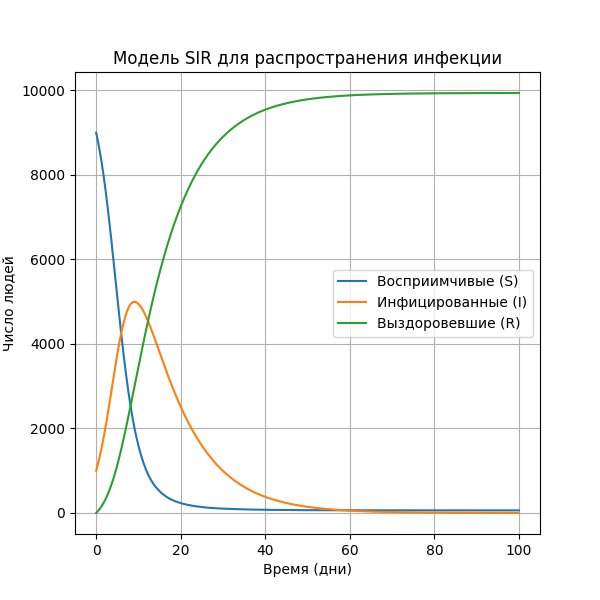
\includegraphics[width=0.76\textwidth]{img/sir_ex(2).png}
	\caption{Динамика численности групп выздоровевших, инфицированных и восприимчивых с течением времени для популяции размером 10000 человек.}
	
	\label{fig:sir}
\end{figure} 
 
Значения параметров, использованных при моделировании приведены в таблице 	\ref{tab:param_th_sir}
 
\begin{table}[h!]
	\centering
	\caption{Таблица значений параметров, использованных для  моделирования в SIR модели.}
	\begin{tabularx}{\textwidth}{|X|X|X|X|}
		\hline
		Параметр & $\beta, (1/\text{дн.})$  & $\mu, (1/\text{дн.})$ & $N, (\text{чел.})$  \\
		\hline
		Значение & $0.5$ & $0.1$ & $10000$  \\
		\hline
	\end{tabularx}
	
	\label{tab:param_th_sir}
\end{table} 
 
 
 
Одним из основных параметров, который описывает распространение инфекции, является базовое репродуктивное число $R_0$. Оно описывает, сколько людей может заразить один инфицированный человек, при условии, что все остальные люди в популяции являются восприимчивыми. В предположении однородности популяции, базовое репродуктивное число может быть найдено следующим образом:

\begin{equation}
	R_0 = \frac{\beta}{\mu}
\end{equation}

Для рассмотренного примера базовое репродуктивное число равно пяти.
\subsection{Модель гетерогенного смешивания}

Модель гетерогенного смешивания в эпидемиологии представляет собой математическую модель, заданную системой дифференциальных уравнений, и описывающую распространение инфекционных заболеваний в неоднородной по числу контактов популяции.

Система уравнений для модели гетерогенного смешивания, использованная в работе, имеет следующий вид:

\begin{equation}
	\begin{cases}
		\frac{d S_k}{d t} = -\lambda_k \beta_0 S_k \Theta(t), \\
		\frac{d I_k}{d t} = -\mu I_k + \lambda_k \beta_0 S_k \Theta(t), \\
		\frac{d R_k}{d t} = \mu I_k \\
		\Theta(t)=\cfrac{\sum_{k} k \lambda_{k} I_{k}(t)}{\sum_{k} k \lambda_{k}} \\
		S(t)=\sum_{k} S_{k} \\
		I(t)=\sum_{k} I_{k} \\
		R(t)=\sum_{k} R_{k} \\
		S_k(t) + I_k(t) + R_k(t) = 1
	\end{cases}
	\label{eq:SIR_system_base_groups}
\end{equation}


где:
\begin{itemize}
	
	\item $S_k(t)$, $S(t)$ -- доля узлов степени k, восприимчивых в момент времени t; общая доля восприимчивых узлов в момент времени t.
	\item$I_k(t)$, $I(t)$ -- доля узлов степени k, инфицированных в момент времени t; общая доля инфицированных узлов	в момент времени t.
	\item $R_k(t)$, $R(t)$ -- доля узлов степени k, выздоровевших в момент времени t; общая доля выздоровевших узлов, в момент времени t.
	\item $\lambda_k$ -- вероятность, с которой узел степени k может быть заражен, если у него есть общие ребра с инфицированными узлами.
	\item $\beta_0$ -- это постоянная скорость, с которой происходит заражение восприимчивых узлов.
	\item $\mu$ -- постоянная скорость, с которой инфицированные узлы выздоравливают.

\end{itemize}

Первое уравнение системы \eqref{eq:SIR_system_base_groups} описывает изменение во времени количества восприимчивых узлов в группе $k$. Оно показывает, что  за счет новых случаев заражения их количество уменьшается со скоростью, которая зависит от скорости распространения инфекции, числа контактов группы $k$, а также числа инфицированных узлов в других группах.

Второе уравнение системы \eqref{eq:SIR_system_base_groups} описывает изменение во времени числа инфицированных узлов в группе $k$. Их количество  увеличивается за счет новых заражений и уменьшается за счет выздоровления ранее инфицированных узлов.
 
Третье уравнение системы \eqref{eq:SIR_system_base_groups} описывает изменение во времени количества выздоровевших узлов в группе $k$. Их количество  увеличивается пропорционально скорости выздоровления и числу инфицированных узлов в группе $k$.

Четвертое уравнение системы \eqref{eq:SIR_system_base_groups} описывает вероятность наличия ребра с инфицированным узлом. При таком подходе эта вероятность одинакова для всех компартментов.

Значение $k$ изменяется от 1 и ограничивается количеством уникальных степеней вершин в графе, формирующем сеть контактов.

\newpage

\section{Сбор данных для городской и сельской местностей}

\subsection{Возрастно-половой состав населения}\label{1}

Для анализа с сайта федеральной службы государственной статистики \cite{rosstat} были взяты данные о числе жителей субъектов РФ по возрастным категориям. В результате для городского и сельского населений были определены их доли от общего числа жителей (Приложение. Таблица \ref{coeff}). Эти значения далее были использованы для создания искусственной популяции. Число мужчин и женщин при этом предлагается рассчитываться по формуле:

\begin{equation}
	{}_n N_x = \alpha_{\text{тип популяции}}^{\text{пол}} \cdot N_{\text{тип популяции}}^{\text{пол}}, 
\end{equation}
где:
\begin{itemize}
	
	\item $n$ -- размер возрастной группы.
	
	\item $x$ -- начало возрастного интервала.
	
	\item $\alpha_{\text{тип популяции}}^{\text{пол}}$ -- доля мужчин/женщин от общего числа мужчин/женщин в зависимости от типа популяции. 
	
	\item $ N_{\text{тип популяции}}^{\text{пол}}$ -- размер выборки для мужчин и женщин в искусственной популяции в зависимости от типа популяции.
	
	
\end{itemize}

По обработанным данным были составлены возрастные пирамиды (Рисунок \ref{fig:tree}).

\begin{figure}[h!]
	\centering
	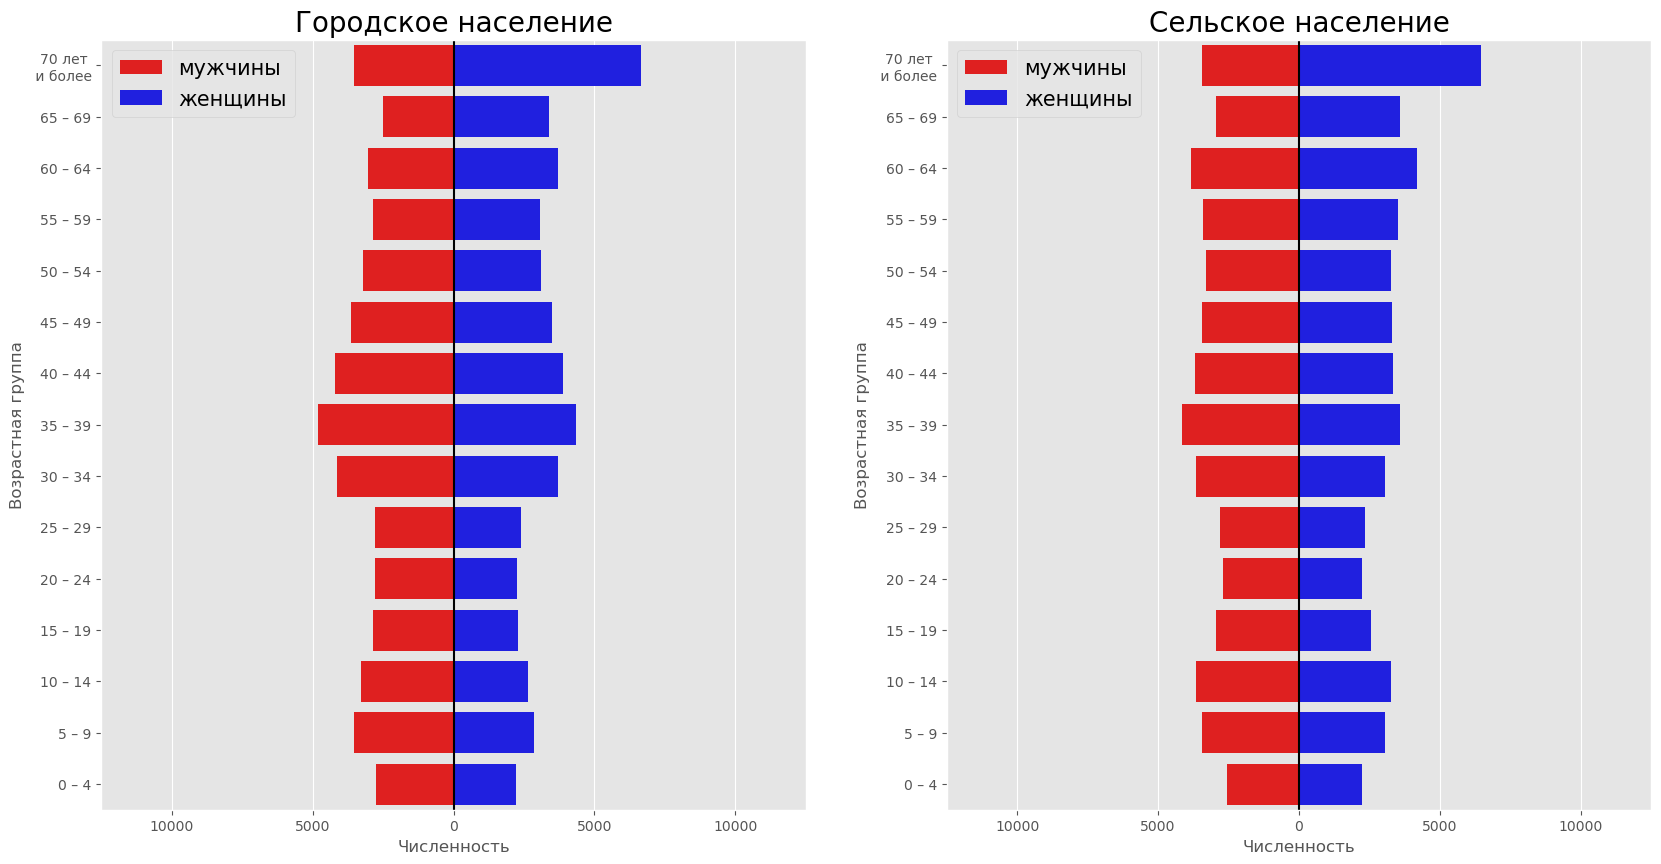
\includegraphics[width=1\textwidth]{img/tree_theory.png}
	\caption{Возрастные пирамиды для сельского и городского населений, построенные по данным Росстата \cite{rosstat}}
	\label{fig:tree}
\end{figure} 

На графике можно видеть, что распределение по возрастам имеет бимодальное распределение. Это может быть связано с тем, что в $90$-е годы в связи с тяжелой обстановкой в стране была низкая рождаемость. Так же можно предположить, что спад обусловлен высокой миграцией молодого населения в те годы. Отдельно можно отметить тот факт, что женщин пожилого возраста больше, чем мужчин как в сельском, так и в городском населении.







\subsection{Предприятия}\label{3}


При построении модели искусственной популяции особое внимание уделялось предприятиям, так как именно на них приходится значительная часть контактов между людьми. Для того, чтобы получить достоверные данные о предприятиях, было проанализировано количество государственных бюджетных учреждений в различных регионах России. При анализе учитывались не только организации, относящиеся к  субъектами РФ, но и муниципальные образования. Таким образом, удалось учесть взаимодействие людей в различных сферах, таких как наука, образование, здравоохранение, культура, социальные услуги и в других областях.


Согласно полученным данным, государственные учреждения распределены по регионам России достаточно равномерно (кроме Москвы). Наибольшее количество таких учреждений находится в Московской области ($1828$ учреждений), в то время как Республика Карелия имеет самое маленькое количество государственных учреждений среди всех регионов -- всего лишь $90$. Этот факт указывает на неравномерность экономического развития регионов, что необходимо учитывать при создании искусственной популяции.

Из данных было установлено, что Московская область сильно отличается по показателям от других областей. Поэтому для анализа того, сколько человек в среднем приходится на одну организацию использовали медиану, так как она не чувствительна к выбросам в данных. 


\subsection{Домохозяйства}\label{5}

При создании искусственной популяции необходимо знать число домохозяйств и их размеры. Это поможет создать более точную и реалистичную сеть контактов, а так же лучше моделировать распространение инфекции. На основе данных Росстата  \cite{rosstat} были получены доли для каждого размера домохозяйств (Рисунок \ref{fig:households_theory1}). В работе рассматривались домохозяйства, включающие от 1 до 6 и более человек. Полученные значения были использованы при дальнейшем математическом моделировании и приведены в приложении, таблица \ref{tab: 111}. 

Из графиков видно, что количество домохозяйств, состоящих из одного человека, в городе значительно больше, чем в селе (в городе $4.1 \cdot 10^7$, в селе -- $1.01 \cdot 10^7$). С ростом числа людей в домохозяйстве разница между городом и селом уменьшается. Так, количество домохозяйств из 6 и более человек для города и села примерно одинаковы и равны $0.2 \cdot 10^7$ и $0.21 \cdot 10^7$ соответственно.


\begin{figure}[h!]
	\centering
	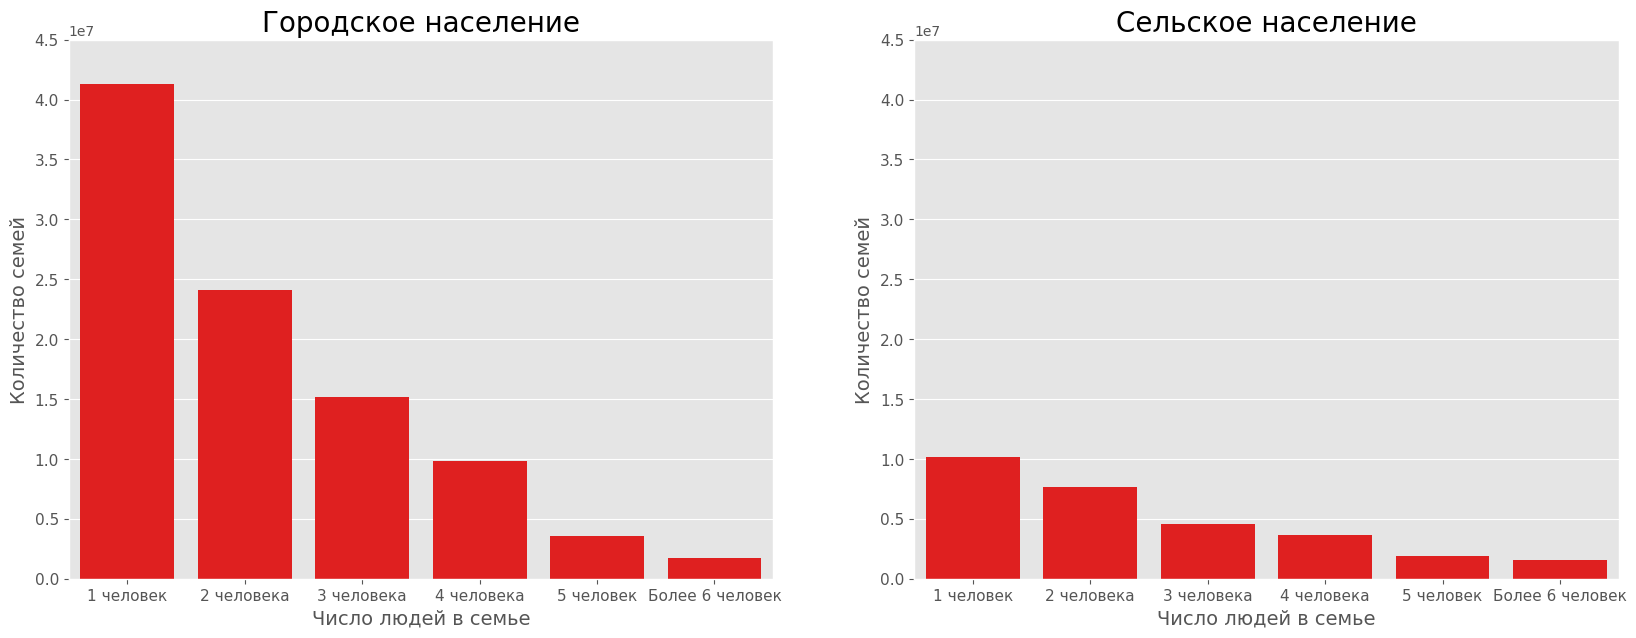
\includegraphics[width=0.99\textwidth]{img/households_distibution_theory.png}
	\caption{Распределение домохозяйств по размерам.}
	\label{fig:households_theory1}
\end{figure}


\subsection{Школы}\label{4}

Отдельно в работе были рассмотрены школы, так как  они являются важным элементом общества не только с точки зрения распространения инфекций, но и с точки зрения использования для математического моделирования различных социальных сценариев, таких как изменение групповой динамики, исследование влияния различных факторов на качество образования и т.д. На графике \ref{fig:schools} приведено количество школ для сельского и городского населений для ряда регионов России.


\begin{figure}[h!]
	\centering
	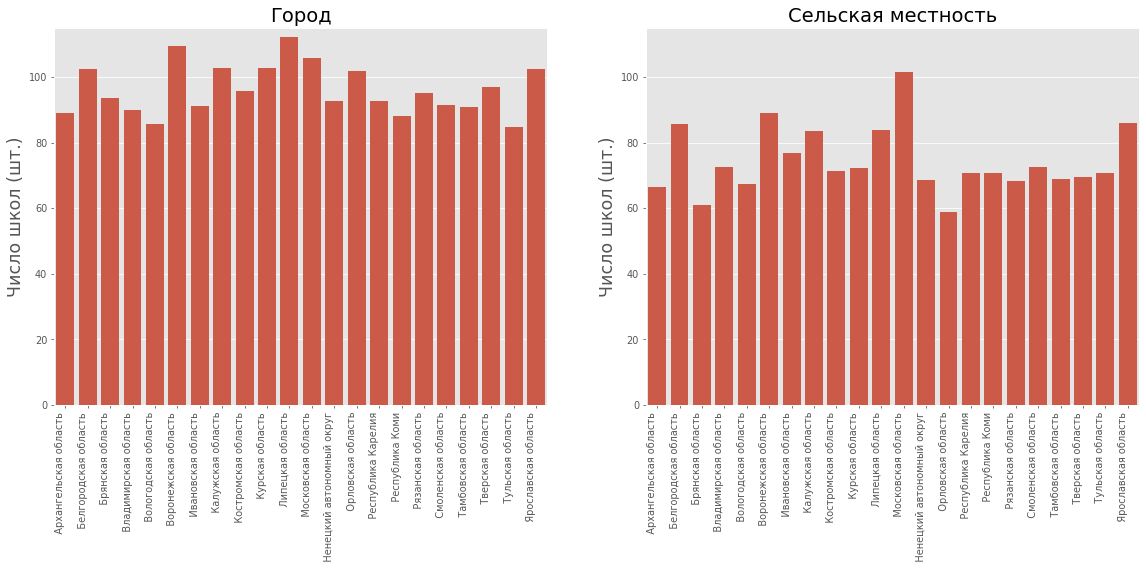
\includegraphics[width=0.99\textwidth]{img/schools.png}
	\caption{Количество школ по субъектам Российской Федерации.}

	\label{fig:schools}
\end{figure}


Из графика видно, что в сельской местности школ меньше чем в городе. При этом анализ результатов расчётов показал, что в среднем для сельского населения на одну школу приходится 18205 человек, для городского – 14689, что может влиять на отличия в динамике распространения инфекции.

\newpage

\section{Алгоритм создания сети контактов}\label{7}
В ходе выполнения работы был разработан и реализован на языке Python алгоритм, позволяющий проводить моделирование распространения инфекции.
Блок-схема алгоритма приведена на рисунке \ref{fig:algo}.

\begin{figure}[h!]
	\centering
	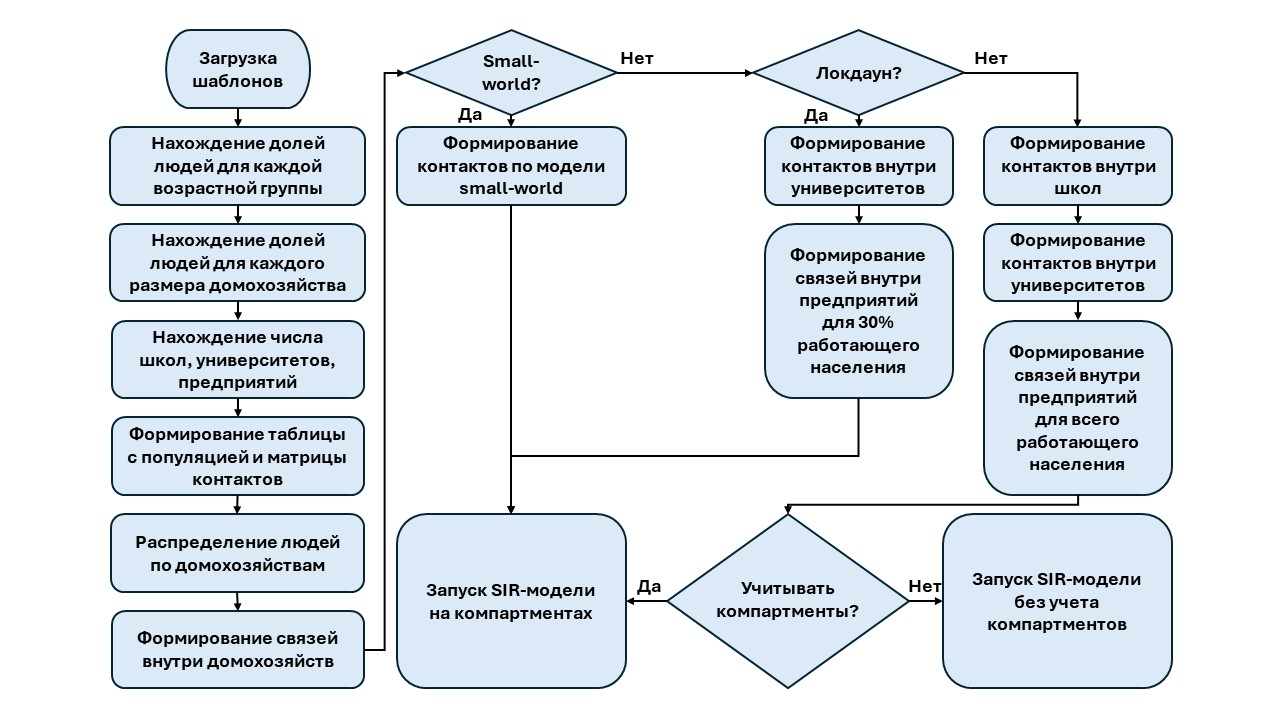
\includegraphics[width=0.96\textwidth]{img/Алгоритм.jpg}
	\caption{Блок-схема работы алгоритма моделирования распространения инфекции.}
	\label{fig:algo}
\end{figure}
 Выполнение алгоритма начинается с считывания и предобработки данных, которые подаются на вход в виде сгруппированных excel файлов.
На их основе рассчитывается, сколько людей должно приходиться на каждую возрастную группу, сколько необходимо создавать школ, университетов и предприятий. Все вычисления проводятся отдельно для городского и сельского населений.
Названия файлов и их описания приведены в приложении, таблица \ref{fig:file}.
В памяти программы популяция хранится в виде таблицы. Список ее полей и их допустимых значений приведены в приложении, таблица \ref{fig:table_paremeters_population}.
Далее идет процесс формирования связей. Здесь выделяются два сценария математического моделирования: с локдауном и без. В обоих случаях информация о контактах хранится в виде разряженной матрицы. При этом в ячейке с индексами i, j содержится 1, если люди с такими id имели контакт, и 0 иначе. Более подробно процесс создания контактов описан в разделе \ref{6}.


\newpage
\section{Создание контактов}\label{6}
\subsection{Домохозяйства}\label{5}
В алгоритме контакты формируются внутри домохозяйств, школ, университетов и предприятий. Данный этап является самым сложным и ресурсозатратным. При этом в каждом случае применяются разные подходы математического моделирования. 

Как уже было описано в разделе \ref{7}, сначала происходит формирование связей внутри домохозяйств. Из таблицы итерационно для каждого размера домохозяйства выбираются люди, которые подходят по возрасту. Между ними в матрице контактов устанавливаются связи, и закрепляется уникальный номер домохозяйства. При этом связи внутри домохозяйства устанавливаются как <<каждый с каждым>>, то есть можно считать, что люди в домохозяйстве образуют полный граф. На рисунке  \ref{fig:households_distibution_generated} приведен результат работы алгоритма по формированию домохозяйств для популяции общим размером 30000 человек.

\begin{figure}[h!]
	\centering
	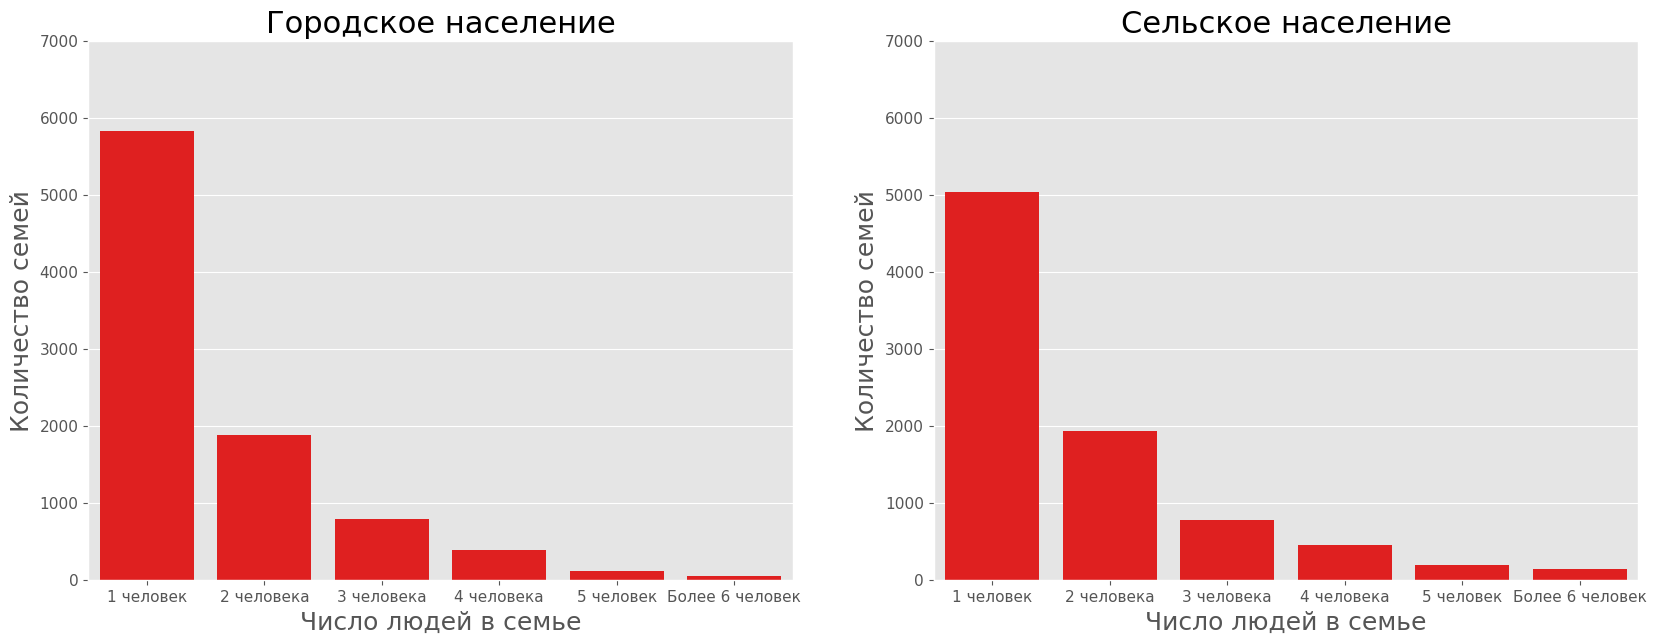
\includegraphics[width=1.\textwidth]{img/households_distibution_generated.png}
	\caption{Распределение домохозяйств для искусственной популяции размером 30000 человек.}
	\label{fig:households_distibution_generated}
\end{figure}

Из графика видно, что распределения размеров домохозяйств имеют тот же характер, что и зависимости, полученные на статистических данных (Рисунок \ref{fig:households_theory1}). Для удобства математического моделирования размеры городской и сельской популяций были приняты равными, поэтому в искусственной популяции нет такого большого различия в количестве семей с малым числом людей в городской и сельской популяции, как это было в распределении на основе статистических данных.


\subsection{Школы и университеты}

Число школ определяется исходя из размера популяции и данных, сформированных на первом этапе работы алгоритма. Контакты внутри школ формируются по модели <<small-world>> \cite{Watts}. Математического моделирование контактов данным алгоритмом происходит отдельно внутри каждого класса. Размер классов устанавливается заранее и не превышает 30 человек. Результат работы алгоритма построения контактов внутри класса приведен на рисунке \ref{fig:graph_connections}.

\begin{figure}[h!]
	\centering
	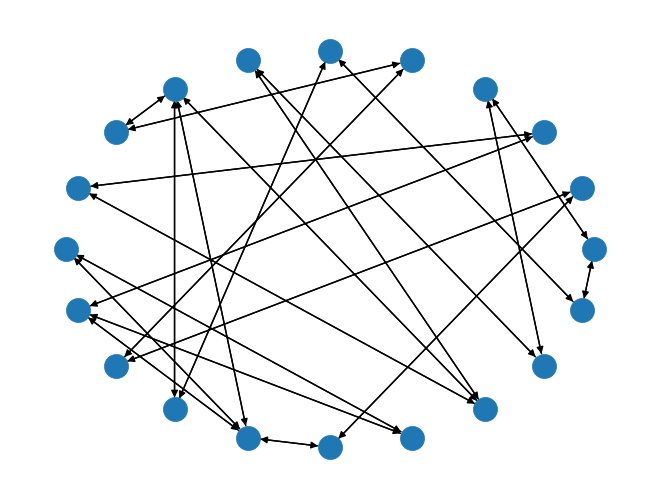
\includegraphics[width=0.5\textwidth]{img/graph_connections.png}
	\caption{Результат работы алгоритма для построения сети контактов внутри класса по модели <<small-world>>. Коэффициент $\beta$ = 0.5.}
	\label{fig:graph_connections}
\end{figure}

Аналогичным образом происходит математическое моделирование контактов внутри университетов, где рассматривается взаимодействие студентов в рамках групп. 


\subsection{Предприятия}

При создании контактов внутри предприятий необходимо учитывать, что все они имеют разный размер. В решения был использован подход описанный в статье \cite{Axtell}. При таком способе моделирования число предприятий убывает с увеличением их размера. Результат работы функции для создания предприятий приведен на рисунке \ref{fig:manufactories_linear}.

\begin{figure}[h!]
	\centering
	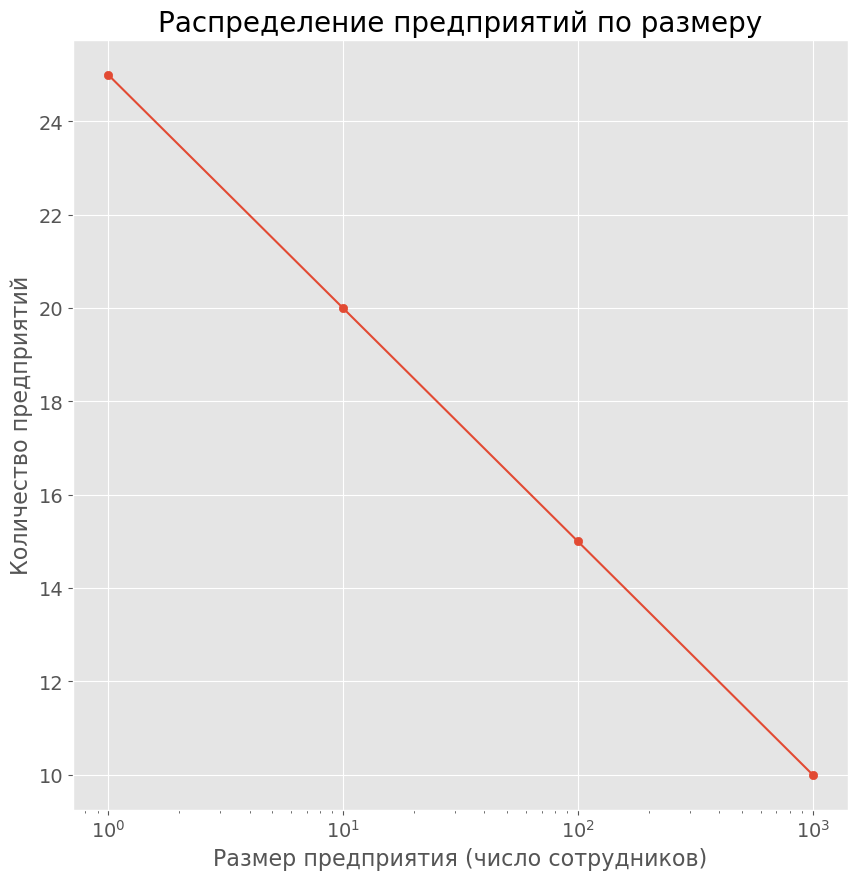
\includegraphics[width=0.7\textwidth]{img/manufactoris_distribution.png}
	\caption{Распределение размеров предприятий по размерам.}
	\label{fig:manufactories_linear}
\end{figure}

Функция создания предприятий на вход получает параметр, который отвечает за то, сколько будет создано самых крупных предприятий. Если с таким число выполнить моделирование невозможно, алгоритм автоматически находит ближайшее допустимое значение к заданному, при этом на экран выводится сообщение с предупреждением.

Помимо этого в программе так же предусмотрен способ моделирования в режиме локдауна. В этом случае считается, что работать на предприятия ходит только 30\% от общего числа трудоспособного населения.

\newpage

\section{Графический анализ результатов работы алгоритма распространения инфекции}

Для анализа результатов работы модели распространения инфекции на матрицах контактов для городского и сельского населений были построены графы. Считается, что каждая вершина графа -- конкретный человек, а ребра -- его контакты. Все вершины были разбиты на подгруппы, исходя из их степени. Гистограммы распределения степеней вершин для городского и сельского населений представлены на рисунке \ref{fig:nodes_degrees}.

\begin{figure}[h!]
	\begin{minipage}{0.5\textwidth}
		\centering
		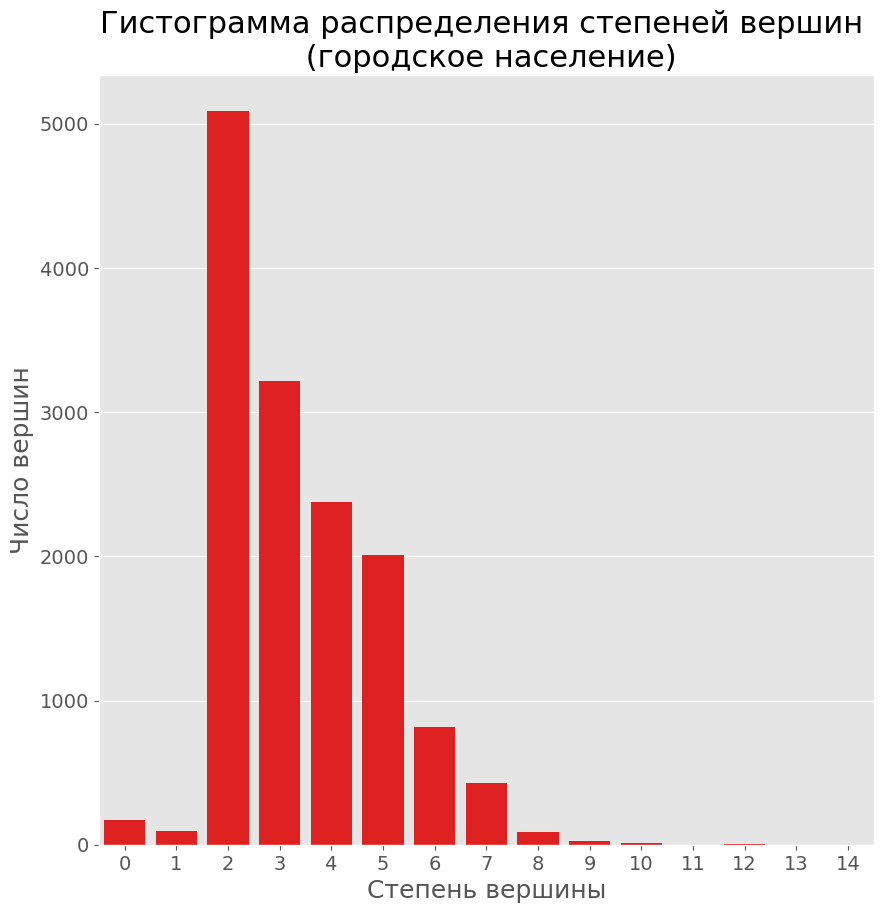
\includegraphics[width=0.99\textwidth]{img/nodes_degrees_urban.png}
	\end{minipage}
	\begin{minipage}{0.5\textwidth}
		\centering
		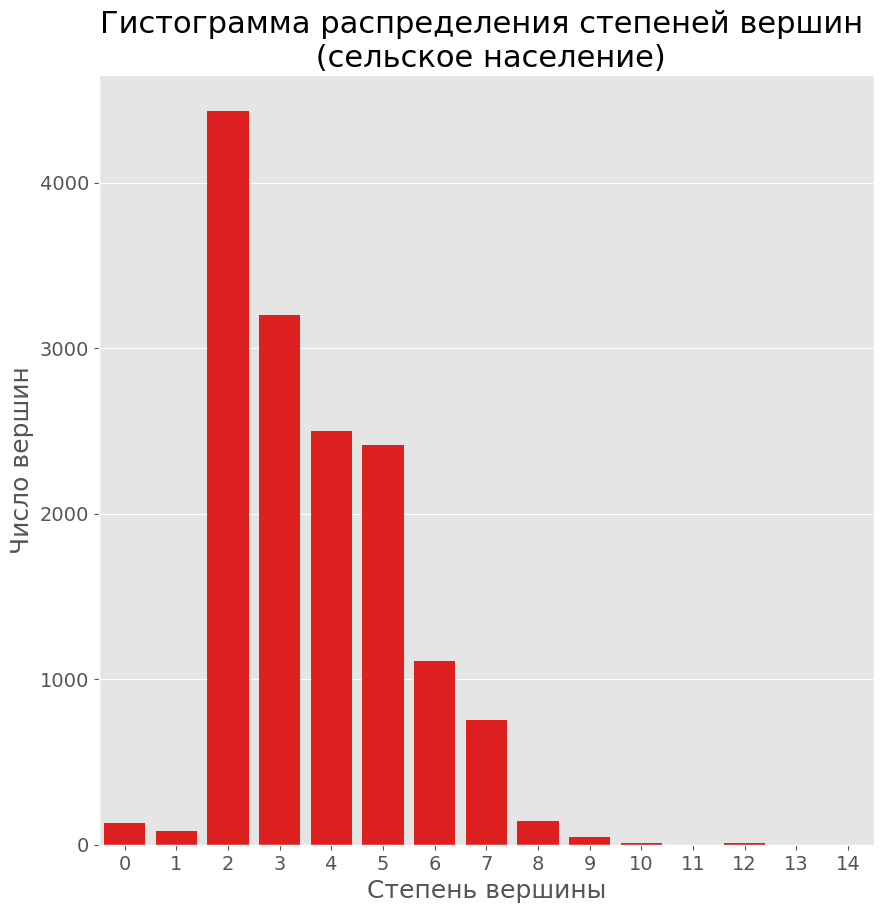
\includegraphics[width=0.99\textwidth]{img/nodes_degrees_rural.png}
	\end{minipage}
	\caption{Распределение степеней вершин сгенерированной популяции для городского и сельского населений.}
	\label{fig:nodes_degrees}
\end{figure}

После этого к полученным подгруппам была применена модель \eqref{eq:SIR_system_base_groups} распространения инфекционного заболевания в популяции. На рисунке \ref{fig:RI} приведены графики изменения числа выздоровевших и инфицированных с течением времени. Параметры, использованные при моделировании, приведены в таблице \ref{tab:param_th}.

\begin{table}[h!]
	\centering
	\caption{Таблица значений параметров, использованных для  моделирования с помощью SIR модели.}
	\begin{tabularx}{\textwidth}{|c|c|c|c|X|}
		\hline
		Параметр & $\gamma,  (1/\text{дн.})$ & $\beta_0,  (1/\text{дн.})$ & Размер популяции, (чел.)& Тип популяции \\
		\hline
		Значение & $1/15$ & $0ю0005$ & $100000$ & Городская \\
		\hline
	\end{tabularx}
	
	\label{tab:param_th}
\end{table}

\begin{figure}[h!]
	\begin{minipage}{0.5\textwidth}
		\centering
		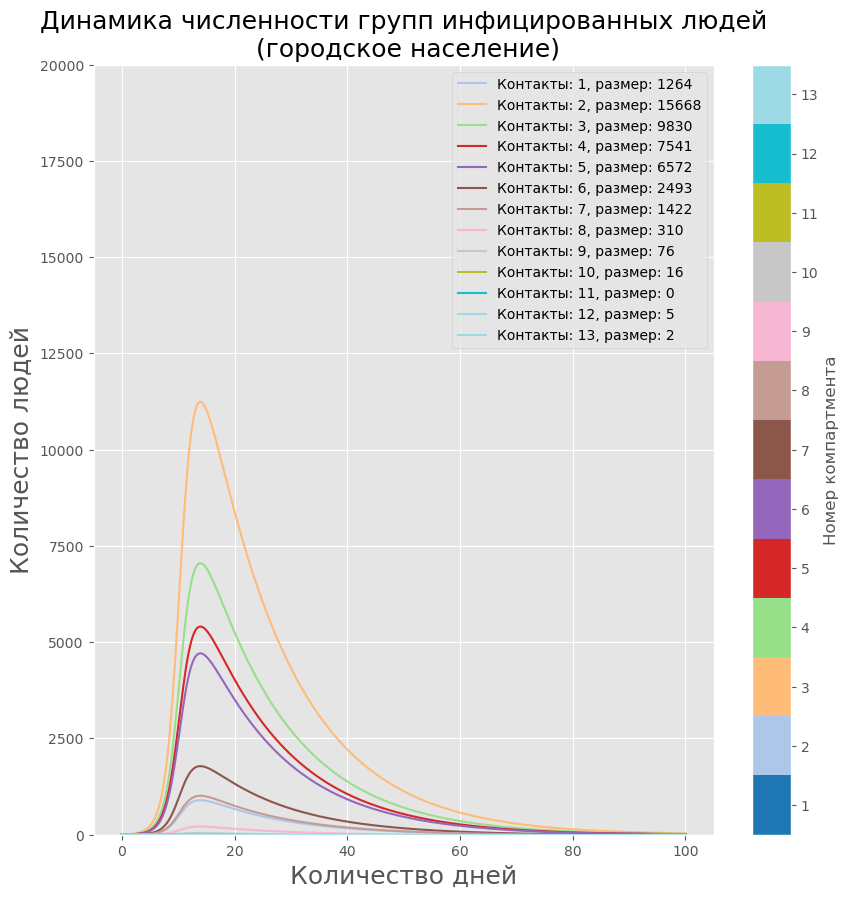
\includegraphics[width=\linewidth]{img/sir_model_compare_I_urban_new.png}
	\end{minipage}
	\begin{minipage}{0.5\textwidth}
		\centering
		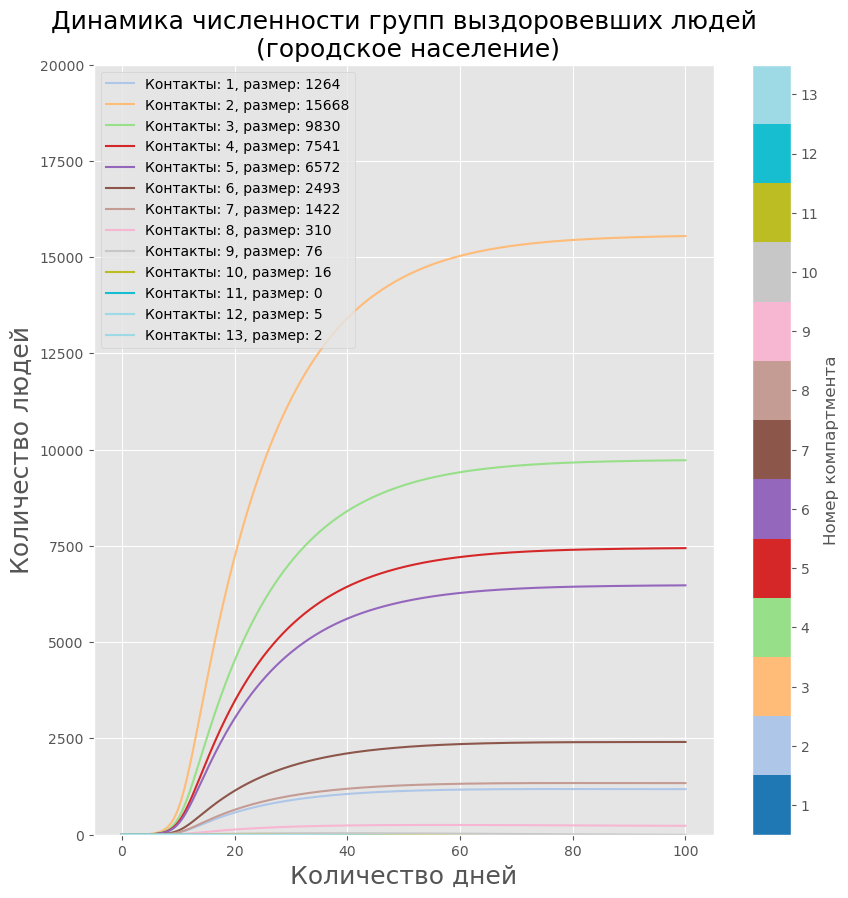
\includegraphics[width=\linewidth]{img/sir_model_compare_R_urban_new.png}
	\end{minipage}
	\caption{Динамика численности групп инфицированных (слева) и выздоровевших (справа) людей для модели с параметрами из таблицы \ref{tab:param_th}.}
	\label{fig:RI}
\end{figure}




Из графиков на рисунке \ref{fig:RI} видно, что характер полученных зависимостей количества заболевших и количества выздоровевших от времени повторяют динамику изменения этих параметров при фактическом течении инфекции. С начала наблюдается значительных рост заболевших, потом их количество начинает снижаться, при этом увеличивается доля выздоровевших.  В результате число инфицированных людей снижается до нуля для каждого компартмента, а количество выздоровевших достигает максимального значения и перестает меняться с течением времени. 

\newpage

\section{Эксперименты}
\subsection{Критерии оценки экспериментов}
Одним из основных терминов при математическом моделировании распространения инфекции является эпидемия. Эпидемия -- это быстрое распространение заболевания среди людей, превышающее обычный уровень заболеваемости на данной территории. Далее под временем присутствия инфекции в популяции будем понимать число дней, через которое количество инфицированных людей упадет до нуля. Под острой фазой эпидемии будем понимать период, в который наблюдается резкий рост функции числа инфицированных. В ходе экспериментов рассчитывались три показателя: время присутствия инфекции в популяции, длительность острой фазы инфекции, процент переболевших людей. Эти показатели позволяют делать оценки об иммунитете населения и результативности принятых мер по борьбе с инфекцией.

Так как в программе присутствуют методы, в основе которых содержится элементы случайности (например, в модели <<small-world>> случайным образом выбираются связи, которые будут разорваны), была предусмотрена возможность фиксации случайного состояния. При  таком подходе результаты работы алгоритма не отличаются от запуска к запуску. Это позволило определять
влияние параметров модели распространения инфекции на результат математического моделирования, при постоянной сети контактов.

\subsection{Сравнение динамики распространения инфекции для сельского и городского населений}

В ходе эксперимента была создана искусственная популяция с параметрами модели, приведенными в таблице \ref{tab:table_paremeters_rural_urban}.
На рисунке \ref{fig:disease_spreading_I} для городского и сельского населений приведены графики изменения численности групп инфицированных людей.  
\begin{table}[h!]
	\centering
	\caption{Таблица значений параметров, использованных для математического моделирования распространения инфекции среди городского и сельского населений.}
	\begin{tabularx}{\textwidth}{|c|c|c|c|X|}
		\hline
		Параметр &  $\gamma,  (1/\text{дн.})$ & $\beta_0,  (1/\text{дн.})$ & Размер популяции, (чел.)& Тип популяции \\
		\hline
		Значение & $1/15$ & $0.0005$ & $100000$ & Городская + Сельская \\
		\hline
	\end{tabularx}
	\label{tab:table_paremeters_rural_urban}
	\vspace{-0.4cm}
\end{table}




\begin{figure}[h!]
	\begin{minipage}{0.5\textwidth}
		\centering
		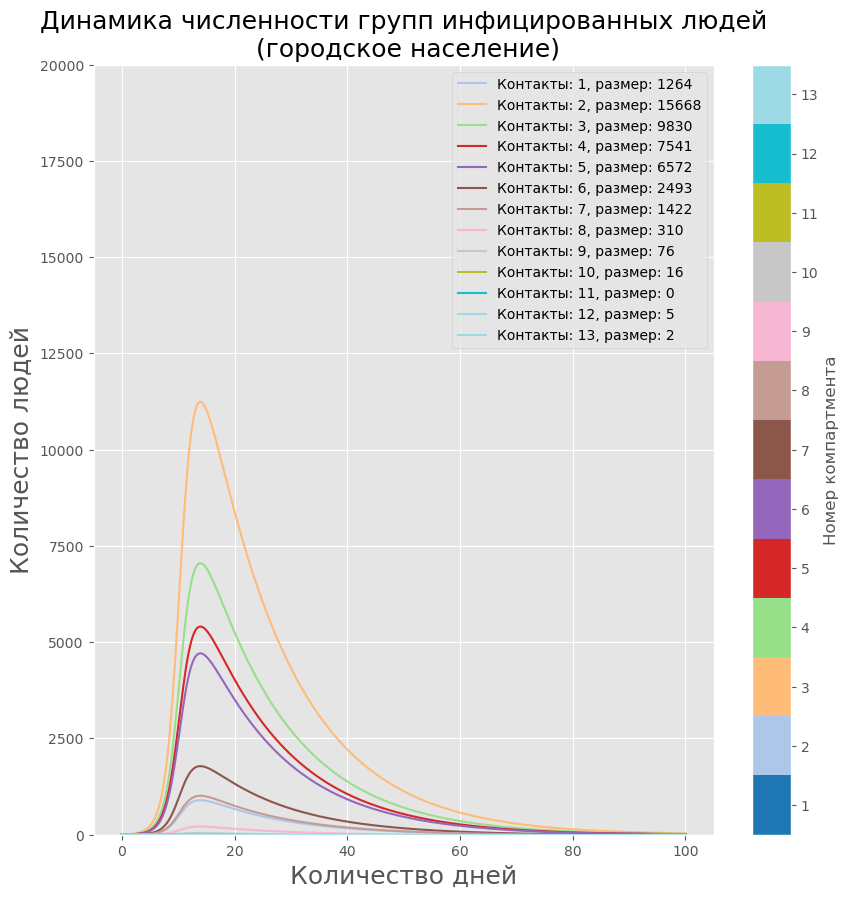
\includegraphics[width=\linewidth]{img/sir_model_compare_I_urban_new.png}
	\end{minipage}
	\begin{minipage}{0.5\textwidth}
		\centering
		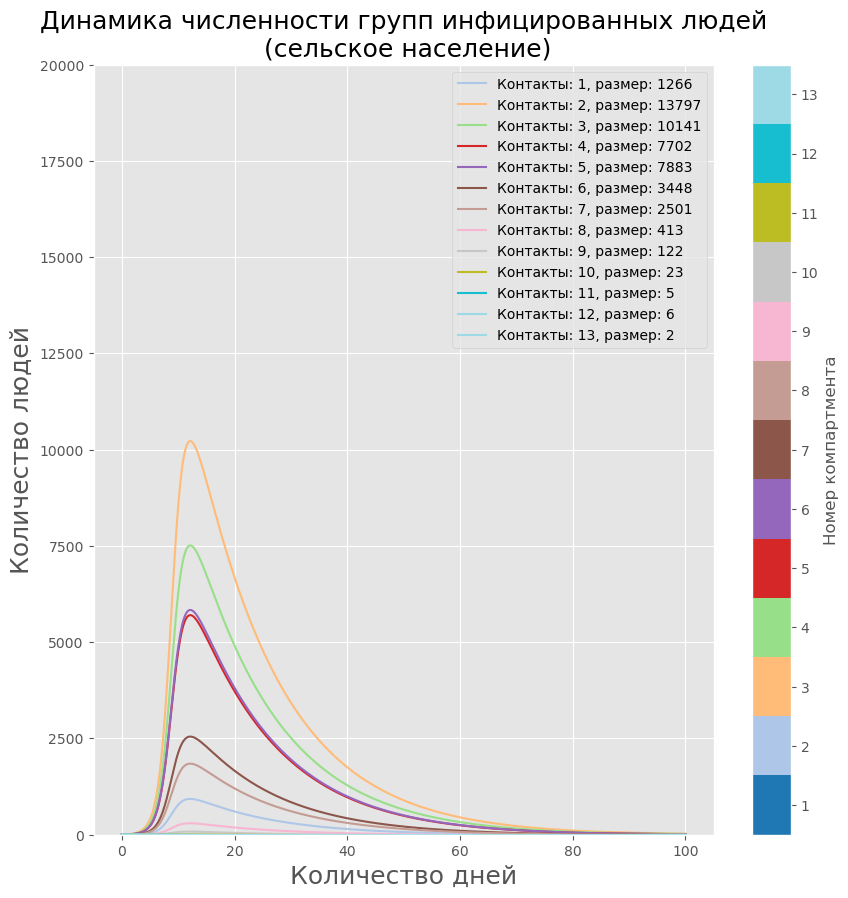
\includegraphics[width=\linewidth]{img/sir_model_compare_I_rural_new.png}
	\end{minipage}
	\caption{Динамика численности групп инфицированных людей с течением времени для городского и сельского населений.}
	\label{fig:disease_spreading_I}
\end{figure}

\begin{comment}
\begin{figure}[h!]
	\begin{minipage}{0.5\textwidth}
		\centering
		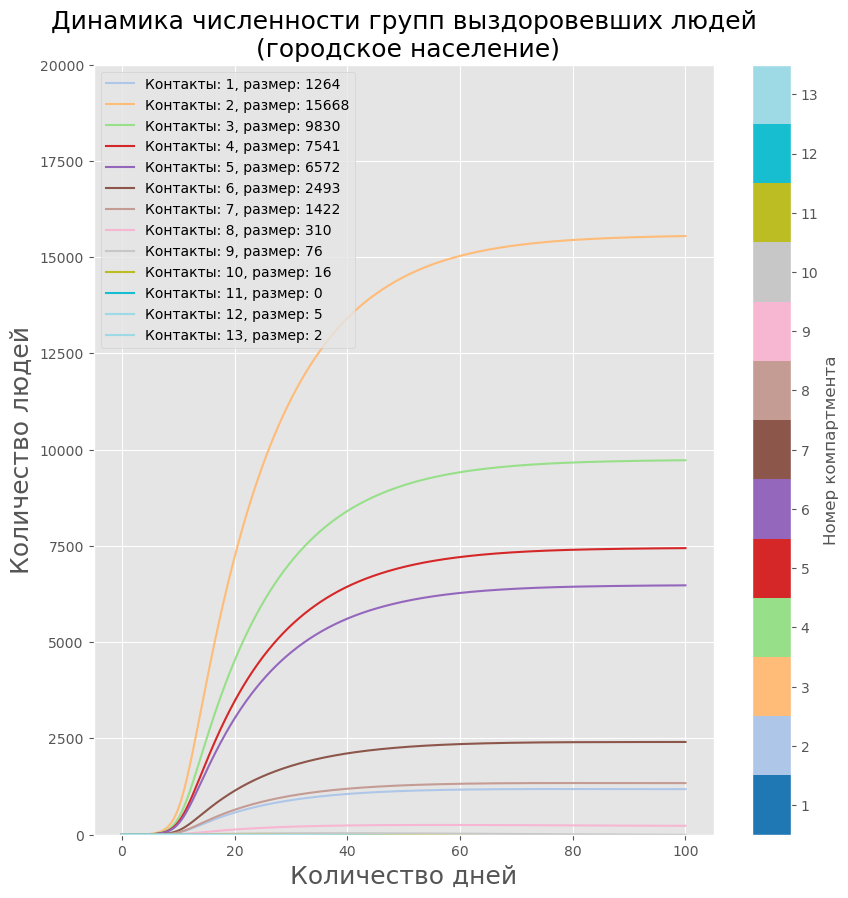
\includegraphics[width=\linewidth]{img/sir_model_compare_R_urban_new.png}
	\end{minipage}
	\begin{minipage}{0.5\textwidth}
		\centering
		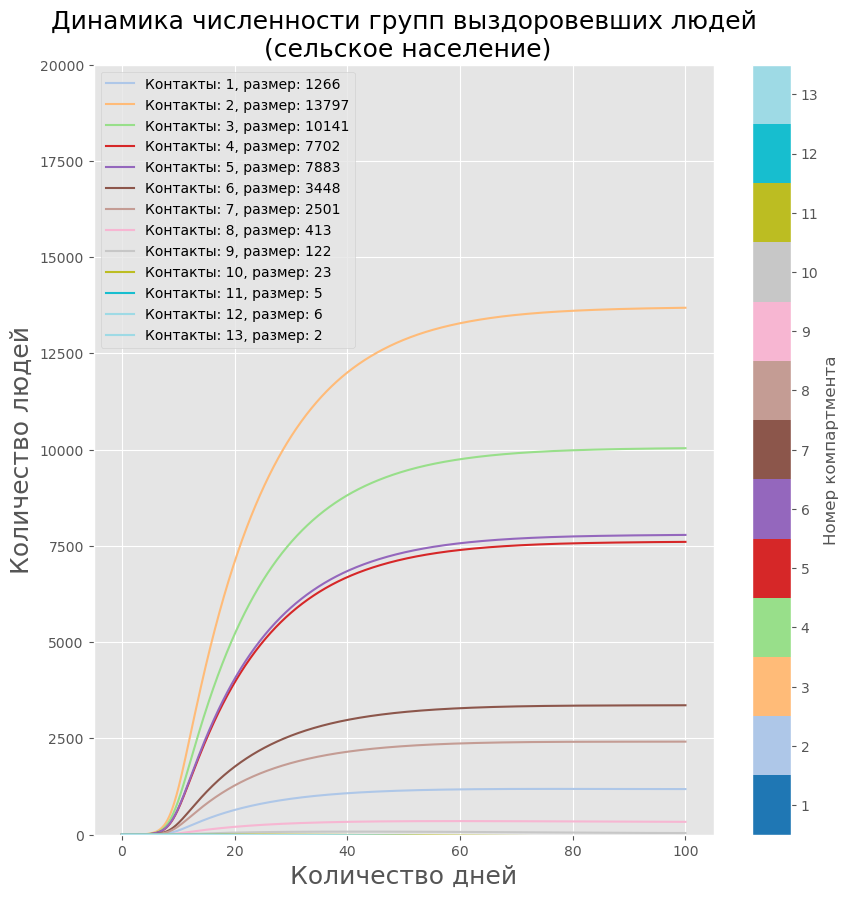
\includegraphics[width=\linewidth]{img/sir_model_compare_R_rural_new.png}
	\end{minipage}
	\caption{Динамика численности групп выздоровевших людей с течением времени для городского и сельского населений.}
	\label{fig:disease_spreading_R}
\end{figure}
\end{comment}


\newpage
В ходе эксперимента для обоих популяций были вычислены следующие метрики: общий процент переболевших людей, средневзвешенное по группам значение количества дней, через которое заканчивается острая фаза эпидемии, время присутствия инфекции в популяции. Полученные значения приведены в таблице \ref{tab:res_compare}.

\begin{table}[h!]
	\centering
	\caption{Таблица значений метрик для городского и сельского населений.}
	\begin{tabularx}{\textwidth}{|X|X|X|}
		\hline
		Метрика & Городское население & Сельское население \\ 
		\hline
		Процент переболевших людей (\%)& 74 & 73 \\ 
		\hline
		Длительность острой фазы эпидемии (дн.) & 12 & 12\\ 
		\hline
		Время присутствия инфекции в популяциии (дн.)& 97 & 98\\ 
		\hline
	\end{tabularx}
	\label{tab:res_compare}
\end{table}

Из полученных данных можно сделать вывод, что для сельского населения эпидемия протекает незначительно, но хуже, чем для городского. Это обусловлено тем, что в среднем для сельского населения характерны более большие семьи, чем для городского (раздел \ref{5}). Кроме того, в сельской местности на одну школу  приходится больше детей, чем в городе (раздел \ref{4}). Это влечет за собой большее число контактов и более быстрое распространение инфекции.


\subsection{Математическое моделирование динамики распространения инфекции при условии локдауна} 

Одним из основных способов борьбы с распространением инфекции является локдаун.
Под локдауном обычно понимается ряд строгих ограничений, которые вводит правительство, с целью предотвращения распространения вируса. Локдаун включает в себя закрытие школ, предприятий, магазинов, запрет на выход на улицу без необходимости.
Прежде всего такие меры помогают снизить количество контактов между людьми и их скопление в общественных местах. В реальных условиях такие меры также помогают медицинской системе снизить нагрузку на больницы и персонал.

В модели наличие локдауна означает, что на предприятия ходят только 30\% трудоспособного населения. Отдельно были рассмотрены численности групп инфицированных и выздоровевших людей с целью оценки динамики распространения инфекции. Параметры, использованные при математическом моделировании, приведены в таблице \ref{tab:table_paremeters_loc_nonloc}. Результаты работы алгоритма приведены на рисунке \ref{fig:disease_spreading_loc_nonloc_I}.

Полученные значения для исследуемых метрик приведены в таблице \ref{tab:res_loc_nonloc}.


\begin{figure}[h!]
	\begin{minipage}{0.5\textwidth}
		\centering
		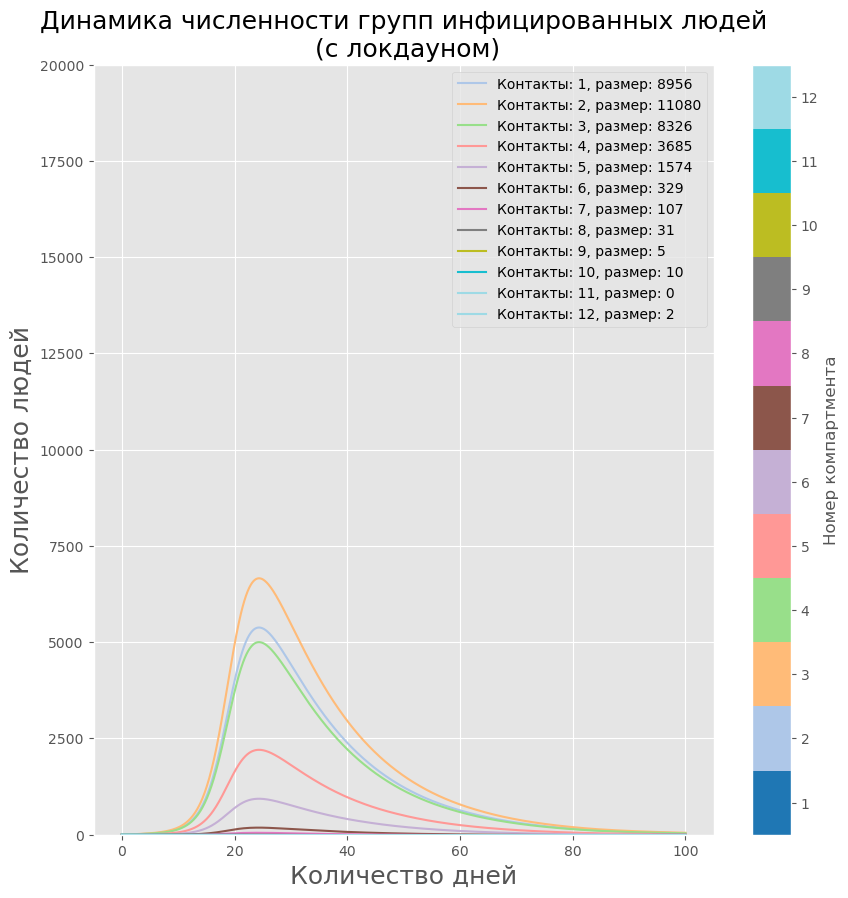
\includegraphics[width=\linewidth]{img/sir_model_lockdown_urban_I_new.png}
	\end{minipage}
	\begin{minipage}{0.5\textwidth}
		\centering
		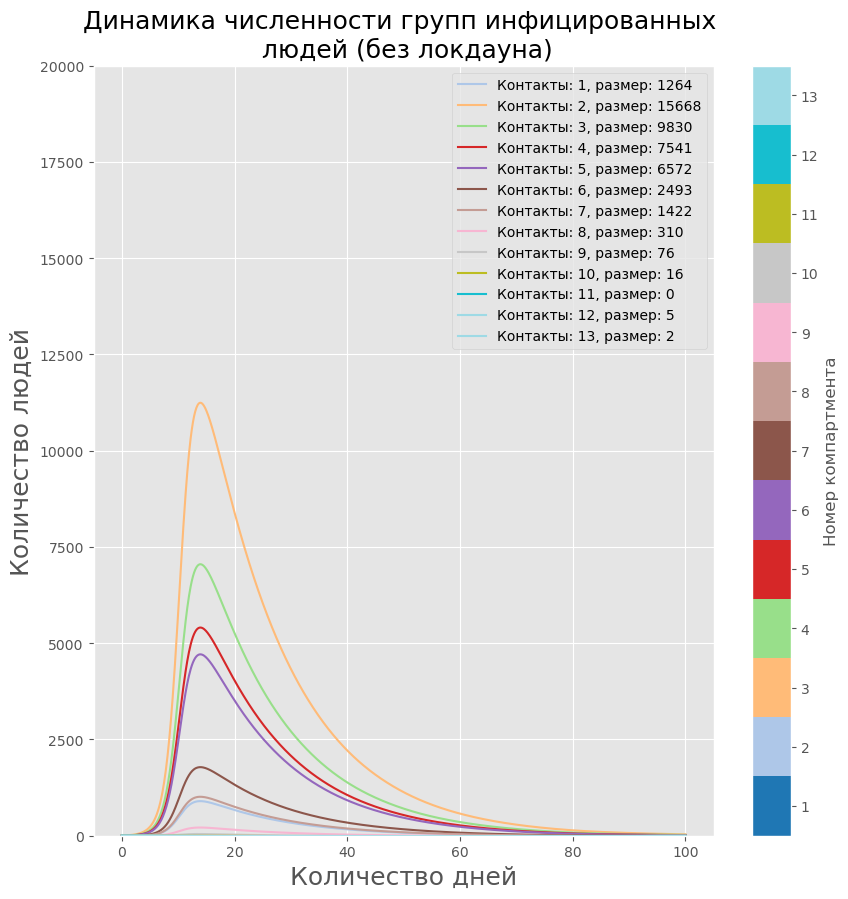
\includegraphics[width=\linewidth]{img/sir_model_nonlockdown_urban_I_new.png}
	\end{minipage}
	\caption{Динамика численности групп инфицированных людей с течением времени при наличии локдауна и без него.}
	\label{fig:disease_spreading_loc_nonloc_I}
\end{figure}

\begin{comment}
\begin{figure}[h!]
	\begin{minipage}{0.5\textwidth}
		\centering
		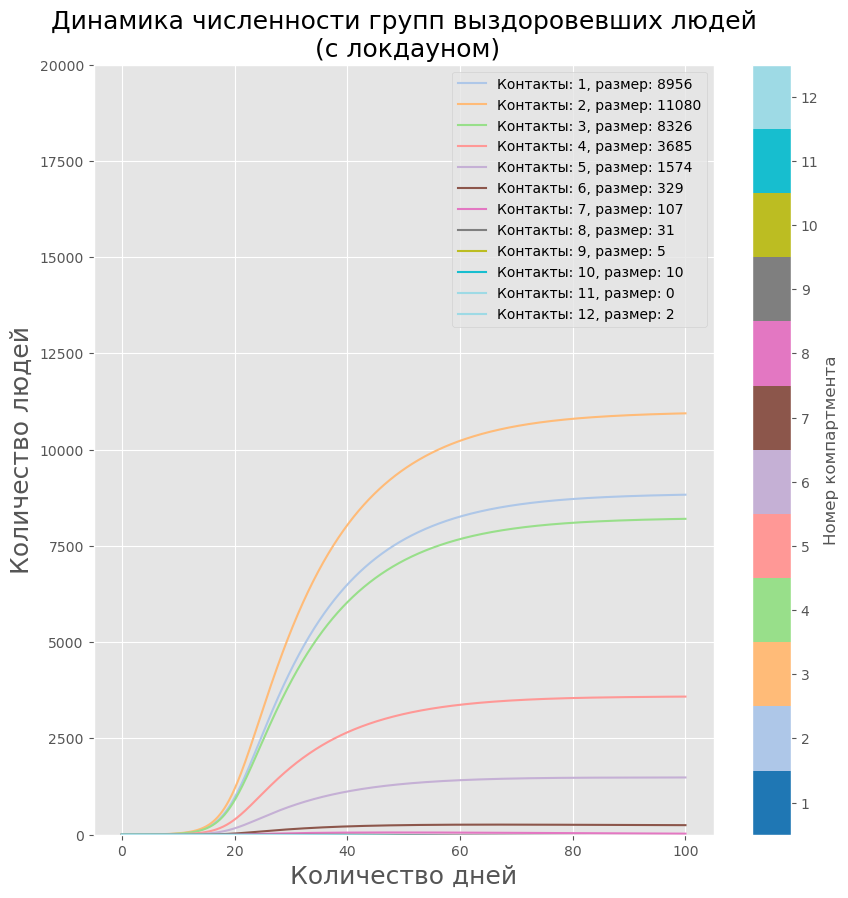
\includegraphics[width=\linewidth]{img/sir_model_lockdown_urban_R_new.png}
	\end{minipage}
	\begin{minipage}{0.5\textwidth}
		\centering
		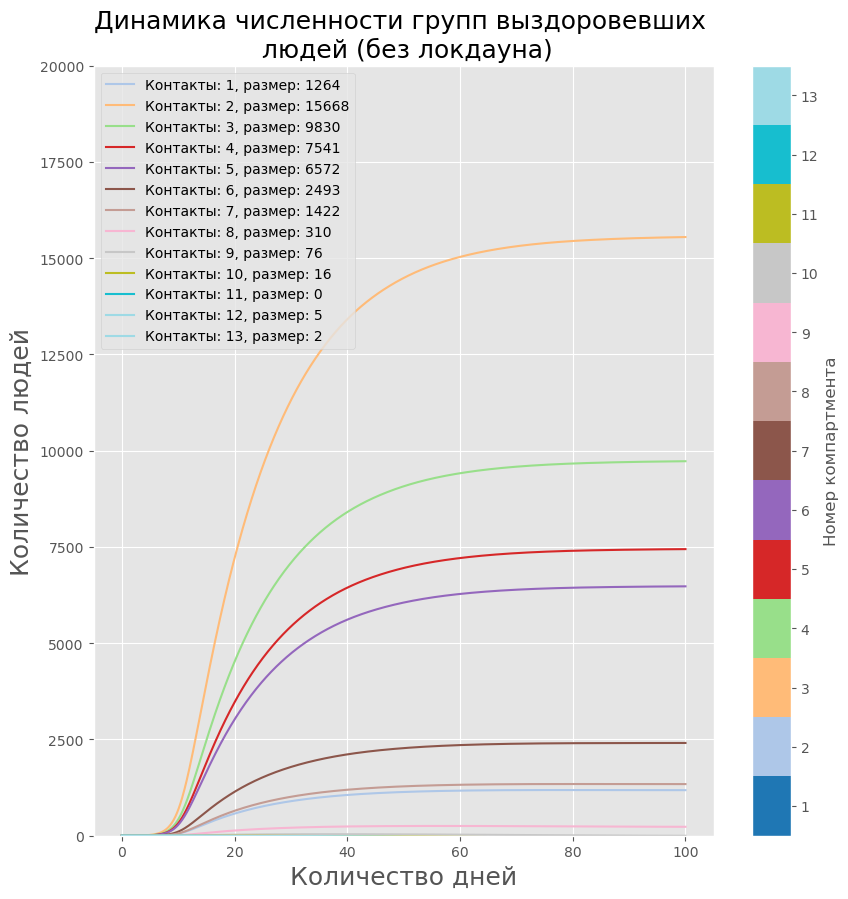
\includegraphics[width=\linewidth]{img/sir_model_nonlockdown_urban_R_new.png}
	\end{minipage}
	\caption{Динамика численности групп выздоровевших людей с течением времени при наличии локдауна и без него.}
	\label{fig:disease_spreading_loc_nonloc_R}
\end{figure}
\end{comment}
\begin{table}[h!]
	\centering
	\caption{Таблица значений параметров, использованных для математического моделирования влияния локдауна на распространение инфекции.}
	\begin{tabularx}{\textwidth}{|c|c|c|c|X|} % X - столбец, который масштабируется
		\hline
		Параметр & $\gamma,  (1/\text{дн.})$ & $\beta_0,  (1/\text{дн.})$ & Размер популяции, (чел.) & Тип популяции \\
		\hline
		Значение & $1/15$ & $0.0005$ & $100000$ & Городская \\
		\hline
	\end{tabularx}
	\label{tab:table_paremeters_loc_nonloc}
\end{table}

\begin{table}[h!]
	\caption{Таблица значений метрик для городского и сельского населений.}
	\centering
	\begin{tabularx}{\textwidth}{|X|X|X|}
		\hline
		Метрика & Без локдауна & С локдауном \\ 
		\hline
		Процент переболевших людей (\%) & 74 & 59 \\ 
		\hline
		Длительность острой фазы эпидемии (дн.) & 12 & 25\\ 
		\hline
     	Время присутствия инфекции в популяции (дн.) & 97 & 98\\ 
		\hline
	\end{tabularx}
	
	\label{tab:res_loc_nonloc}
\end{table}

\newpage
Результаты проведенного эксперимента демонстрируют, что введение локдауна существенно снижает процент переболевших людей (с 74\% до 59\%). Это подтверждает эффективность локдауна как меры для контроля распространения заболевания. Однако несмотря на это значительное уменьшение заболеваемости, время присутствия инфекции в популяции остаётся неизменными, что говорит о необходимости применения дополнительных мер для более полного и эффективного воздействия на распространение инфекции, например, вакцинирование или ношение масок.


\subsection{Математическое моделирование динамики распространения инфекции на сети контактов, построенной по методу small-world} 

В этом эксперименте вся сеть контактов формировалась с помощью подхода <<small-world>>.
На рисунке \ref{fig:small_world_graphics} приведены графики изменения численности групп инфицированных (слева) и выздоровевших (справа) с течением времени. В таблице \ref{tab:table_paremeters_small_world} приведены параметры, с которыми проводилось математическое моделирование. В таблице \ref{tab:results_small_world} приведены значения исследуемых метрик. 

\begin{figure}[h!]
	\begin{minipage}{0.5\textwidth}
		\centering
		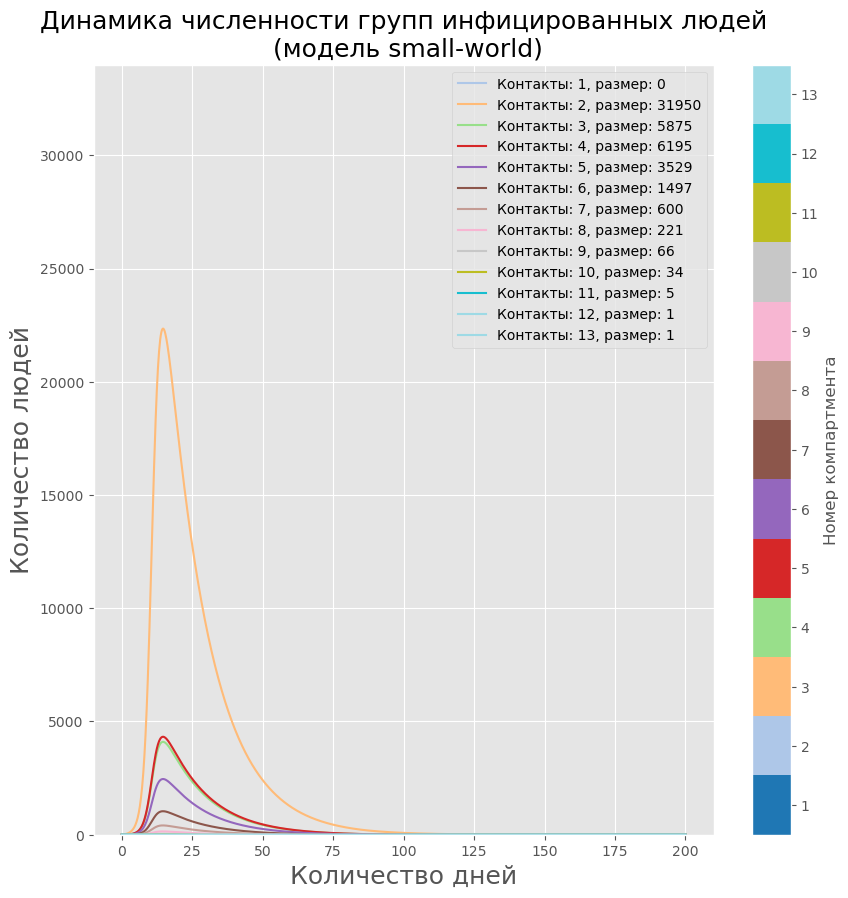
\includegraphics[width=\linewidth]{img/sir_model_small_world_I_rural_new.png}
	\end{minipage}
	\begin{minipage}{0.5\textwidth}
		\centering
		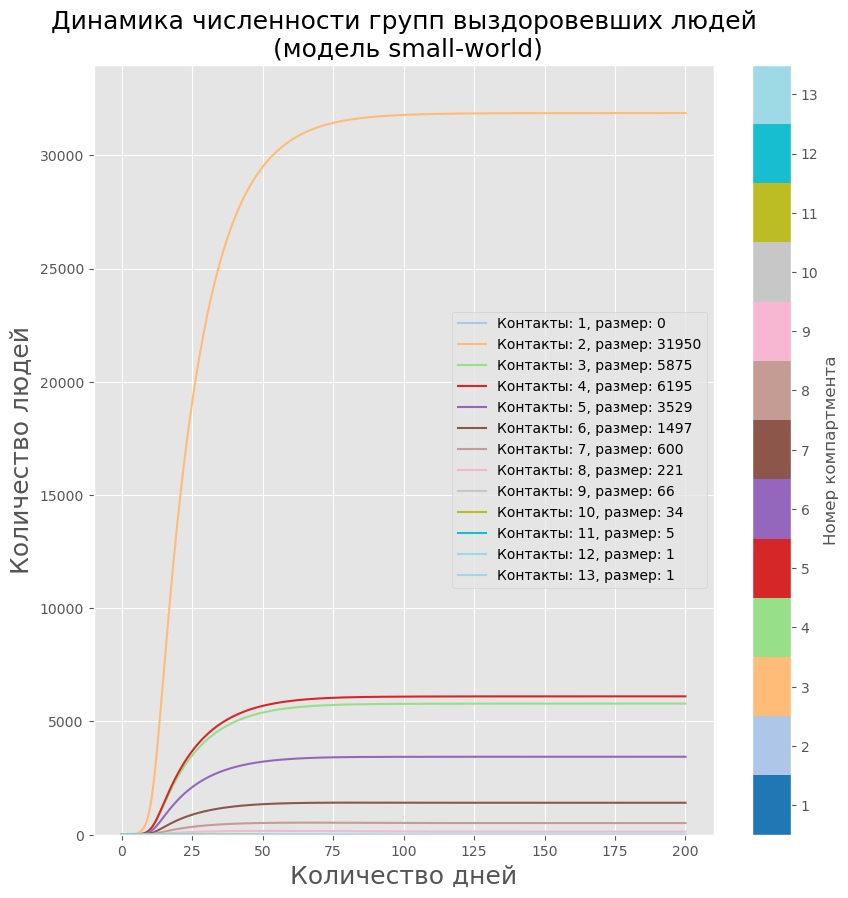
\includegraphics[width=\linewidth]{img/sir_model_small_world_R_rural_new.png}
	\end{minipage}
	\caption{Динамика размера групп инфицированных и выздоровевших людей с течением времени для сети контактов, полученной с помощью подхода small-world.}
	\label{fig:small_world_graphics}
\end{figure}

\begin{table}[h!]
	\centering
	\caption{Таблица значений параметров, использованных для математического моделирования распространение инфекции на сети контактов, построено по принципу small-world.}
	\begin{tabularx}{\textwidth}{|c|c|c|c|X|}
		\hline
		Параметр &  $\gamma,  (1/\text{дн.})$ & $\beta_0,  (1/\text{дн.})$ & Размер популяции, (чел.) & Тип популяции \\
		\hline
		Значение & $1/15$ & $0.0005$ & $100000$ & Городская \\
		\hline
	\end{tabularx}
	\label{tab:table_paremeters_small_world}
\end{table}

\begin{table}[h!]
	\centering
	\caption{Таблица значений метрик математического моделирования с подходом small-world.}
	\begin{tabularx}{\textwidth}{|X|X|}
		\hline
		Метрика & Значение \\ 
		\hline
		Процент переболевших людей (\%)& 70 \\ 
		\hline
		Длительность острой фазы эпидемии (дн.) & 14 \\ 
		\hline
		Время присутствия инфекции в популяции (дн.) & 160 \\ 
		\hline
	\end{tabularx}
	\label{tab:results_small_world}
\end{table}

В ходе проведенного эксперимента отмечается явное увеличение заболеваемости в группе, где индивиды имеют два контакта (Рисунок  \ref{fig:small_world_graphics}). Этот результат объясняется тем, что при инициации математического моделирования по принципу <<small-world>> предполагается, что все члены общества располагаются в круг и образуют кольцо связей. В данном эксперименте вероятность разрыва и переноса связей в графе контактов составляла 0.2. Такое же значение было использовано для установления контактов внутри классов и учебных групп. Однако применение данного подхода ко всей популяции привело к значительному дисбалансу в группе людей с двумя контактами. Это указывает на то, что константу нельзя рассматривать как универсальную для всех размеров групп, и настройка алгоритма должна производиться с учетом специфики задачи.



\subsection{Математическое моделирование динамики распространения инфекции с помощью модели распространения инфекционного заболевания в популяции без учета числа контактов индивидов} 

В эксперименте вся сеть контактов формировалась так же, как и в случае математического моделирования распространения инфекции без ввода локдауна. Отличительной особенностью математического моделирования являлось то, что модель распространения инфекционного заболевания в популяции применялась сразу ко всей сети без учета компартментов. При этом в качестве параметра $\lambda_k$ бралось среднее значение по всем компартментам.
В таблице \ref{tab:table_paremeters_no_comp} приведены параметры, с которыми проводилось математического моделирование. В таблице \ref{tab:results_no_comp} приведены полученные значения  метрик. На рисунке \ref{fig:small_world_graphics_no_comp} приведены графики изменения численности групп инфицированных, выздоровевших и восприимчивых людей с течением времени.


\begin{figure}[h!]
		\centering
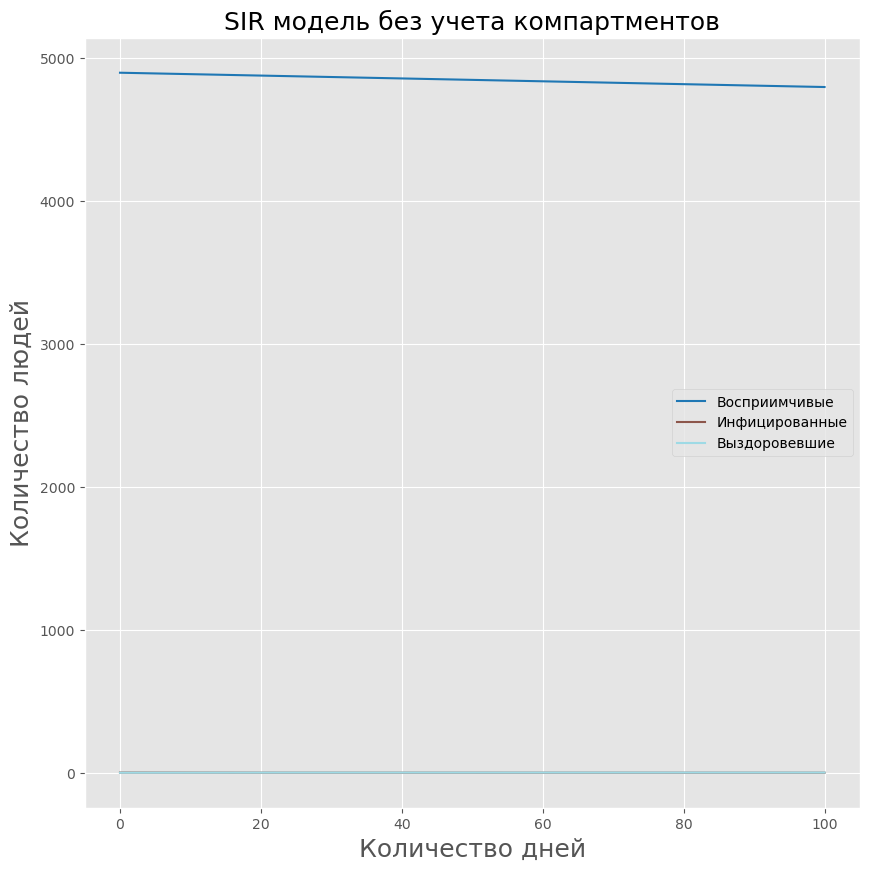
\includegraphics[width=0.5\textwidth]{img/sir_to_all.png}
\caption{Динамика изменения численности групп выздоровевших, инфицированных и восприимчивых для модели, примененной ко всей популяции.}
\label{fig:small_world_graphics_no_comp}
\end{figure}



\begin{table}[h!]
	\centering
		\caption{Таблица значений параметров, использованных для математического моделирования распространение инфекции на сети контактов без учета компартментов.}
	\begin{tabularx}{\textwidth}{|c|c|c|c|X|}
		\hline
		Параметр & $\gamma,  (1/\text{дн.})$ & $\beta_0, (1/\text{дн.})$ & Размер популяции, (чел.)& Тип популяции \\
		\hline
		Значение & $1/15$ & $0.0005$ & $100000$ & Городская \\
		\hline
	\end{tabularx}
	\label{tab:table_paremeters_no_comp}
\end{table}

\begin{table}[h!]
	\centering
	\caption{Таблица значений метрик математического моделирования с подходом small-world.}
	\begin{tabularx}{\textwidth}{|X|X|}
		\hline
		Метрика & Значение  \\ 
		\hline
		Процент переболевших людей (\%)& 92 \\ 
		\hline
		Длительность острой фазы эпидемии (дн.) & 2 \\ 
		\hline
	    Время присутствия инфекции в популяции (дн.) & 101 \\ 
		\hline
	\end{tabularx}
	\label{tab:results_no_comp}
\end{table}

В результате эксперимента наблюдался значительно более быстрый рост числа инфицированных людей, чем при математическом моделировании распространения инфекции на компартментах. Это означает, что при переходе к математическому моделированию на всей популяции необходимо производить корректировку параметров модели. Например, параметра скорости распространения инфекции. В эксперименте была получена зависимость процента переболевших от значения параметра скорости распространения инфекции  (Рисунок \ref{fig:sir_beta}).


\begin{figure}[h!]
	\centering
\vspace{-0.6cm}
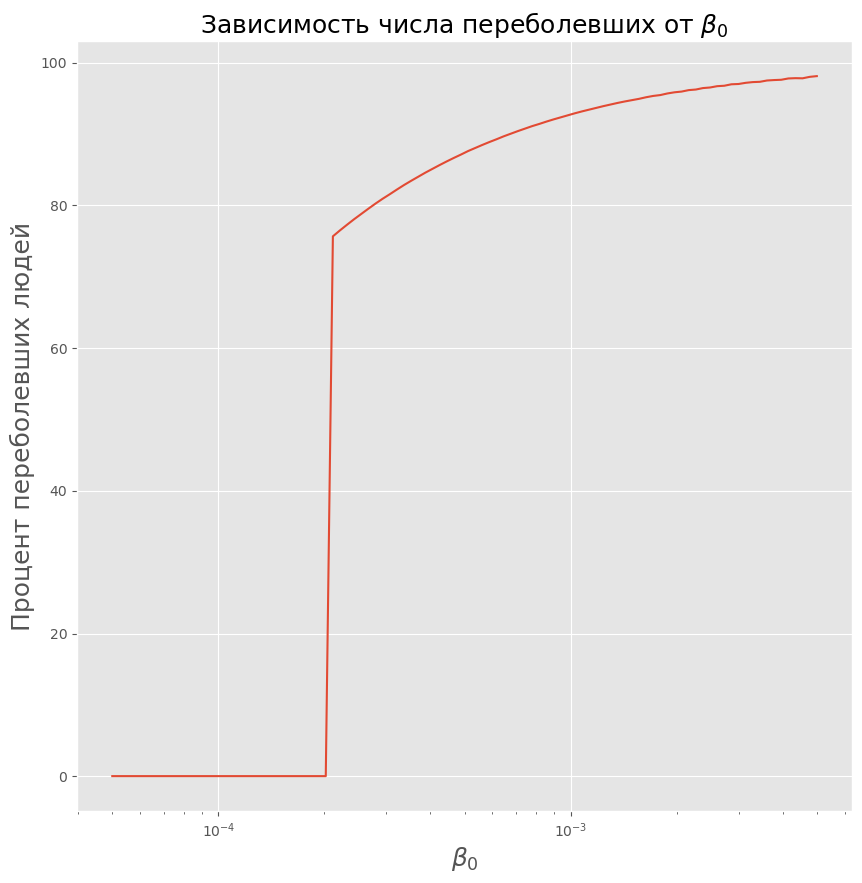
\includegraphics[width=0.5\textwidth]{img/sir_beta.png}
\caption{График зависимости процента переболевших людей от скорости распространения инфекции.}
	\label{fig:sir_beta}
\end{figure}

 При увеличении скорости распространения инфекции, увеличивается процент переболевших людей. Так изменение скорости от 0.0005 до 0.005 приводит с росту процента переболевших от 84\% до 96\%.


\newpage



\section{Заключение}

Целью работы являлось исследование влияние свойств сети контактов на динамику эпидемиологического процесса при помощи компартменто-сетевой модели. Для достижения цели были решены следующие задачи:

\begin{enumerate}
	\item Разработан алгоритм построения сети контактов для жителей городской и сельской местностей на основе демографических и социо-эконономических данных о населении Российской Федерации. Алгоритм позволяет учесть большое количество информации о свойствах реальной популяции, позволяет проводить моделирование на различных сетях контактов и в разных условиях.  
	Программная реализация алгоритма была выполнена на языке Python и имеет модульную структуру. Основными модулями программы являются: модуль загрузки данных, модуль создания сети контактов, расчетный модуль, а также модуль графического интерфейса.

	\item  Реализована компартментно-сетевая модель для описания распространения респираторной инфекции в популяциях городского и сельского типов. 
	Решение системы дифференциальных уравнений, описывающих модель, производилось методом численного интегрирования с использованием python-библиотеки scipy. Использованный метод является надежным и позволяет быстро решать системы линейных дифференциальных уравнений с заданной точностью.
	 
	\item Промоделировано распространение инфекции в популяциях с различными типами сетей контактов. Всего было выполнено пять экспериментов.  Во всех экспериментах рассчитывались три основные метрики: время присутствия инфекции в популяции, длительность острой фазы эпидемии, процент переболевших людей от общего размера популяции.
\end{enumerate}


Сравнение результатов экспериментов показало, что подходы, основанные на компартментно-сетевых моделях, не уступают теоретическим подходам, таким как small-world. 

В ходе экспериментов было установлено, что результаты работы алгоритма на сети контактов small-world сильно зависят от константы, которая отвечает за вероятность переброса ребра в сети контактов. Это видно из рисунка \ref{fig:small_world_graphics}, на котором наблюдается сильный рост числа инфицированных индивидов для группы с двумя контактами. Это связано с тем, что вероятность переброса ребра $\beta$ = 0.2 оказалось слишком маленькой, что привело к большому размеру компартмента индивидов с двумя связями и повлияло на скорость заражения внутри этого компартмента.

Также получено, что при использовании SIR модели необходимо производить точную настройку параметра скорости распространения инфекции. Это видно из рисунка \ref{fig:small_world_graphics_no_comp}: при применении SIR модели ко всей популяции с параметрами, которые использовались при моделировании на компарментах, длительность острой фазы инфекции составляет всего два дня. Например, согласно исследованию \cite{Adhikari}, длительность острой фазы инфекции при COVID-19 составляла от 7 до 20 дней. Поэтому перед решением практических задач, требуется проводить настройку модели под текущие условия.

Результаты расчётов подтвердили эффективность локдауна, как меры по борьбе с распространением инфекции. В результате эксперимента процент переболевших людей снизился с 74\% до 59\%. В реальных условиях это позволило бы снизить нагрузку на медицинские учреждения и их персонал.

Сравнение динамики распространения инфекции для городского и сельского населения не выявили серьезных различий, это видно из рисунка \ref{fig:disease_spreading_I}. В перспективе, для проведения дополнительного сравнительного анализа распространения инфекции в городской и сельской местности можно, например, рассмотреть гипотезу о том, что в сельской местности люди пожилого возраста перестают работать, а в городе продолжают. Принятие этой гипотезы уточнит получаемые результаты.



\newpage 

\begin{thebibliography}{99}
	\bibitem{Murray} Murray J. D., Murray J. D. Epidemic models and the dynamics of infectious diseases //Mathematical biology. – 1993. – С. 610-650.
	\bibitem{Tomsk} Ajelli M., Litvinova M. Estimating contact patterns relevant to the spread of infectious diseases in Russia //Journal of theoretical biology. – 2017. – Т. 419. – С. 1-7.
	
	\bibitem{network_analysis} Klovdahl A. S. et al. Social Networks in an Urban Area: First Canberra Study1 //The Australian and New Zealand Journal of Sociology. – 1977. – Т. 13. – №. 2. – С. 169-172.
	
	\bibitem{Klovdahl} Klovdahl A. S. et al. Social Networks in an Urban Area: First Canberra Study1 //The Australian and New Zealand Journal of Sociology. – 1977. – Т. 13. – №. 2. – С. 169-172.
	
	\bibitem{Eubank} Eubank S. et al. Modelling disease outbreaks in realistic urban social networks //Nature. – 2004. – Т. 429. – №. 6988. – С. 180-184.
	
	\bibitem{Meyers} Meyers L. A. et al. Network theory and SARS: predicting outbreak diversity //Journal of theoretical biology. – 2005. – Т. 232. – №. 1. – С. 71-81.
	
	\bibitem{Meyers_2003} Meyers L. A. et al. Applying network theory to epidemics: control measures for Mycoplasma pneumoniae outbreaks //Emerging infectious diseases. – 2003. – Т. 9. – №. 2. – С. 204.
	
	\bibitem{Halloran} Halloran M. E. et al. Containing bioterrorist smallpox //Science. – 2002. – Т. 298. – №. 5597. – С. 1428-1432.
	
	\bibitem{BA} Barabási A. L., Albert R. Emergence of scaling in random networks //science. – 1999. – Т. 286. – №. 5439. – С. 509-512.
	
	\bibitem{Watts}	Watts D. J., Strogatz S. H. Collective dynamics of ‘small-world’networks //nature. – 1998. – Т. 393. – №. 6684. – С. 440-442.
	
	\bibitem{www} Jeong A. H. Diameter of the world-wide web //Nature. – 1999. – Т. 401. – С. 130-131.
	
	\bibitem{Wuchty}
	Wuchty S. Scale-free behavior in protein domain networks //Molecular biology and evolution. – 2001. – Т. 18. – №. 9. – С. 1694-1702.
	
	\bibitem{rosstat} https://rosstat.gov.ru/
	
	\bibitem{Axtell} Axtell R. L. Zipf distribution of US firm sizes //science. – 2001. – Т. 293. – №. 5536. – С. 1818-1820.
	
	\bibitem{Moreno}
	Moreno Y., Pastor-Satorras R., Vespignani A. Epidemic outbreaks in complex heterogeneous networks //The European Physical Journal B-Condensed Matter and Complex Systems. – 2002. – Т. 26. – С. 521-529
	
	\bibitem{Bansal}
	Bansal S., Grenfell B. T., Meyers L. A. When individual behaviour matters: homogeneous and network models in epidemiology //Journal of the Royal Society Interface. – 2007. – Т. 4. – №. 16. – С. 879-891.
	
	
	\bibitem{Keeling}
	Keeling M. J. The effects of local spatial structure on epidemiological invasions //Proceedings of the Royal Society of London. Series B: Biological Sciences. – 1999. – Т. 266. – №. 1421. – С. 859-867.
	
	\bibitem{Luke}
	Luke D. A., Harris J. K. Network analysis in public health: history, methods, and applications //Annu. Rev. Public Health. – 2007. – Т. 28. – С. 69-93.
	
	\bibitem{Sun}
	Sun Y., Han J. Mining heterogeneous information networks: principles and methodologies. – Morgan \& Claypool Publishers, 2012.

	\bibitem{Adhikari}
	Adhikari S. P. et al. Epidemiology, causes, clinical manifestation and diagnosis, prevention and control of coronavirus disease (COVID-19) during the early outbreak period: a scoping review //Infectious diseases of poverty. – 2020. – Т. 9. – С. 1-12.

	\bibitem{voz}
	http://gp91.ru/f/kontaktnye\_dlya\_saita\_kopiya.pdf

\end{thebibliography}


\newpage


\section{Приложение}


\begin{table}[h]
	\centering
	\caption{ Таблица файлов, которые алгоритм использует для расчета.}
	\begin{tabularx}{\textwidth}{|c|X|}
		\hline
		Название файла & Описание \\ 
		\hline
		age\_sex\_distribution\_percentage.xlsx & Файл представляет из себя таблицу, в которой указано, сколько процентов от всей популяции составляют люди каждой возрастной группы. \\ 
		\hline
		households.xlsx & Файл содержит размеры домохозяйств для всех регионов страны. \\ 
		\hline
		manufactures.xlsx & Файл содержит информацию о числе предприятий разных видов для каждой области. \\ 
		\hline
		schools.xlsx & Файл содержит информацию о том, сколько школ приходится на каждую область. \\ 
		\hline
	\end{tabularx}
	\label{fig:file}
\end{table}



\begin{table}[h]
	\centering
	\caption{Таблица допустимых значений параметров для популяции.}
	\begin{tabularx}{\textwidth}{|c|X|}
		\hline
		Параметр               & Допустимые значения                                         \\
		\hline
		Id                     & целочисленное значение (integer). -1 если не заполнено      \\
		Возраст                & целочисленное значение (integer). -1 если не заполнено      \\
		Пол                    & male/female                                                 \\
		Id домохозяйства       & целочисленное значение (integer). -1 если не заполнено      \\
		Социальная роль        & ребенок/родитель/не имеет детей                             \\
		Тип популяции          & сельская/городская                                                 \\
		Номер предприятия      & целочисленное значение (integer). -1 если не заполнено      \\
		Номер университета     & целочисленное значение (integer). -1 если не заполнено      \\
		\hline
	\end{tabularx}
	\label{fig:table_paremeters_population}
\end{table}


\definecolor{lightblue}{RGB}{153,204,255}
\definecolor{darkblue}{RGB}{51,102,204}

\begin{table}[h!]
	\centering
	\setlength{\arrayrulewidth}{1pt}
	\renewcommand{\arraystretch}{1.5}
	\caption{Таблица коэффициентов $\alpha$ по возрастным группам для города и сельской местности.}
	\begin{tabularx}{\linewidth}{|X|X|X|X|X|}
		\hline
		{Возрастная группа} & 
		{Мужчины (город)} &
		{Женщины (город)} &
		{Мужчины (село)}   &
		{Женщины (село)} \\
		\hline
		0 – 4 & 0.048228 & 0.038131 & 0.041090 & 0.035985 \\ \hline
		05 – 9 & 0.065078 & 0.051348 & 0.057092 & 0.049954 \\ \hline
		10 - 14 & 0.060426 & 0.047758 & 0.057801 & 0.050684 \\ \hline
		15 - 19 & 0.057738 & 0.043964 & 0.048541 & 0.041152 \\ \hline
		20 - 24 & 0.052066 & 0.039552 & 0.044843 & 0.034962 \\ \hline
		25 - 29 & 0.055083 & 0.046135 & 0.051216 & 0.040149 \\ \hline
		30 - 34 & 0.087438 & 0.075185 & 0.078978 & 0.063005 \\ \hline
		35 - 39 & 0.094538 & 0.083253 & 0.084348 & 0.069109 \\ \hline
		40 - 44 & 0.084593 & 0.076494 & 0.077282 & 0.066098 \\ \hline
		45 - 49 & 0.075172 & 0.070111 & 0.074774 & 0.067012 \\ \hline
		50 - 54 & 0.062727 & 0.061496 & 0.072401 & 0.067978 \\ \hline
		55 - 59 & 0.062977 & 0.068045 & 0.082824 & 0.082579 \\ \hline
		60 - 64 & 0.067163 & 0.081208 & 0.091281 & 0.097663 \\ \hline
		65 - 69 & 0.054906 & 0.075574 & 0.065990 & 0.081770 \\ \hline
		70 - 74 & 0.038728 & 0.060998 & 0.039667 & 0.059454 \\ \hline
		75 - 79 & 0.013435 & 0.025484 & 0.011941 & 0.024921 \\ \hline
		80 - 84 & 0.013622 & 0.035173 & 0.013374 & 0.040230 \\ \hline
		85 и более & 0.006083 & 0.020092 & 0.006556 & 0.027296 \\
		\hline
	\end{tabularx}
	\label{coeff}
\end{table}


\definecolor{lightblue}{RGB}{153,204,255}
\definecolor{darkblue}{RGB}{51,102,204}

\begin{table}[h!]
	\centering
	\setlength{\arrayrulewidth}{1pt}
	\renewcommand{\arraystretch}{1.5}
	\caption{Таблица коэффициентов $\beta$  работающих людей по возрастным группам для города и сельской местности.}
	\begin{tabularx}{\linewidth}{|X|X|X|X|X|}
		\hline
		{Возрастная группа} &
		{Работающие городские мужчины} &
		{Работающие сельские мужчины}  & 
		{Работающие городские женщины} &
		{Работающие сельские женщины}  \\ \hline
		15-19 & 0.007213 & 0.007326 & 0.007216 & 0.007605 \\ \hline
		20-29 & 0.151962 & 0.153703 & 0.130307 & 0.132786 \\ \hline
		30-39 & 0.304655 & 0.283241 & 0.284305 & 0.265716 \\ \hline
		40-49 & 0.261809 & 0.252996 & 0.284548 & 0.287475 \\ \hline
		50-59 & 0.190951 & 0.223993 & 0.207252 & 0.235805 \\ \hline
		60-69 & 0.075921 & 0.074554 & 0.076101 & 0.064979 \\ \hline
		70-74 & 0.005512 & 0.003359 & 0.007223 & 0.004248 \\ \hline
		75 and over & 0.001977 & 0.000827 & 0.003048 & 0.001386 \\ \hline
	\end{tabularx}
	\label{coeffааа}
\end{table}


\definecolor{lightblue}{RGB}{153,204,255}
\definecolor{darkblue}{RGB}{51,102,204}

\begin{table}[h!]
	\centering
	\setlength{\arrayrulewidth}{1pt}
	\renewcommand{\arraystretch}{1.5}
		\caption{Размеры домохозяйств для городского и сельского населений, усредненные по регионам страны.}
	\begin{tabularx}{\linewidth}{|X|X|X|}
		
		\hline
		{Размер домохозяйства, (число человек)} &
		{Доля от общего числа домохозяйств для сельского населения, (\%)} &
		{Доля от общего числа домохозяйств для сельского населения, (\%)} \\
		\hline
		1 & 34.5 & 43.2  \\
		\hline
		2 & 25.8 & 25.2  \\
		\hline
		3 & 15.6 & 15.8  \\
		\hline
		4 & 12.2 & 10.3  \\
		\hline
		5 & 6.4 & 3.6  \\
		\hline
		более 6 & 5.5 & 1.9  \\
		\hline
	\end{tabularx}
	\label{tab: 111}
\end{table}







\end{document}

